\section{Results}\label{sec:results}

\subsection{The model can be fitted to convergence, but its posterior is bimodal}\label{sec:res-fit}

\paragraph{Convergence.}
The first question is whether the estimators can be fitted to convergence and whether their posteriors are identified (\Cref{tab:fit}).
Every posterior-mode fit converged: after Newton polishing the largest gradient component of any stored optimum is \nMapGradMax{} and the smallest Hessian eigenvalue is \nMapHessMin{}, so every optimum is a strict local maximum.
The dominant-mode NUTS fits of Family-HB converge for every quantity the likelihood identifies (class weights, annotator rates, credibilities): maximum $\widehat{R}$ \nNutsRhatIdMin{}--\nNutsRhatIdMax{} and minimum bulk effective sample size \nNutsEssIdMin{}--\nNutsEssIdMax{} across the four universes, with at most \nNutsDivMax{} divergent transition.
The only sites with $\widehat{R}$ above \nRhatFlag{} are coordinates of the hierarchical prior in the global fit, family means and non-centred annotator offsets (maximum \nNutsRhatAllGlob{}, bulk ESS \nNutsEssAllGlob{}), which the likelihood constrains only through the annotator rates they combine into; no identified quantity is flagged, and among the per-mode runs used for bridge sampling below only that of the global second mode, whose posterior probability is negligible, is flagged on identified quantities.
Posterior-mode and posterior-mean credibilities agree closely (Spearman correlation at least \nMvnSpMin{}; Jaccard index of the Strong sets \nMvnJacMin{}--\nMvnJacMax{}), and the posterior-mode credibility of every edge lies inside its 95\% credible interval.
Posterior uncertainty nevertheless matters at the margin (post hoc summary): of the edges with posterior mean credibility above 0.5, \nNutsStradGlob{} of \nNutsGtHalfGlob{} in the global universe and \nNutsStradImm{} of \nNutsGtHalfImm{} in the immune universe have a 95\% credible interval that includes 0.5.
% provenance: paper/r2/tables/tab_fit.tex generated by src/r2/paper_assets on 2026-10-15 04:06 from data/r2/tables/
%   fit_convergence.csv (modified 2026-10-14 19:28): fit_id in {family_hb, family_hb_nuts}
%   fit_map_optima.csv (modified 2026-10-14 19:28): fit_id == family_hb & optimum == 1
%   modes_bridge.csv (modified 2026-10-14 20:11): role == primary_estimate & mode == 1; role == raw_noncentred_coordinates (bridge check in the non-centred coordinates)
%   fit_class_weights.csv (modified 2026-10-14 19:28): fit_id == family_hb_nuts & class_name == T
\begin{table}[tbp]
\centering
\small
\setlength{\tabcolsep}{4pt}
\caption{Family-HB fit diagnostics per universe: posterior-mode search, mass of the second optimum, convergence of the dominant-mode NUTS run and the class weight of true edges.}
\label{tab:fit}
\begin{tabular}{@{}lrrrr@{}}
\toprule
 & Global & Immune & Kidney & Lung \\
\midrule
\multicolumn{5}{@{}l}{\emph{Posterior mode (multi-start MAP)}} \\
Observation patterns $P$ & 20{,}278 & 3{,}388 & 2{,}440 & 3{,}170 \\
Restarts & 50 & 50 & 50 & 50 \\
Distinct optima & 2 & 2 & 3 & 4 \\
Restarts at the best optimum & 27 & 29 & 29 & 12 \\
Gap to second optimum (log post.) & 108.3 & 7.5 & 7.9 & 11.6 \\
Second-mode prob., Laplace & $3.9\times 10^{-46}$ & 0.0016 & 0.0073 & $8.9\times 10^{-5}$ \\
Second-mode prob., bridge sampling$^{\dagger}$ & \begin{tabular}[t]{@{}c@{}}$1.8\times 10^{-46}$\\[-1pt]{\scriptsize [$1.1\times 10^{-46}$, $3.1\times 10^{-46}$]}\end{tabular} & \begin{tabular}[t]{@{}c@{}}0.0044\\[-1pt]{\scriptsize [0.0028, 0.0069]}\end{tabular} & \begin{tabular}[t]{@{}c@{}}0.0029\\[-1pt]{\scriptsize [0.0018, 0.0048]}\end{tabular} & \begin{tabular}[t]{@{}c@{}}$6.3\times 10^{-5}$\\[-1pt]{\scriptsize [$3.9\times 10^{-5}$, $1.0\times 10^{-4}$]}\end{tabular} \\
\quad range (draw sets, proposals)$^{\dagger}$ & \begin{tabular}[t]{@{}r@{}}$1.8\times 10^{-46}$--\\$2.1\times 10^{-46}$\end{tabular} & \begin{tabular}[t]{@{}r@{}}0.0044--\\0.0085\end{tabular} & \begin{tabular}[t]{@{}r@{}}0.0022--\\0.0041\end{tabular} & \begin{tabular}[t]{@{}r@{}}$6.3\times 10^{-5}$--\\$7.3\times 10^{-5}$\end{tabular} \\
\addlinespace[3pt]
\multicolumn{5}{@{}l}{\emph{Full posterior (NUTS, dominant mode; 4 chains $\times$ 1{,}000 draws)}} \\
Max.\ $\widehat{R}$, all sites & 1.016 & 1.009 & 1.009 & 1.007 \\
Max.\ $\widehat{R}$, identified sites & 1.004 & 1.003 & 1.004 & 1.006 \\
Min.\ bulk ESS, all sites & 300 & 752 & 848 & 649 \\
Min.\ bulk ESS, identified sites & 1{,}951 & 1{,}676 & 1{,}921 & 1{,}710 \\
Divergent transitions & 0 & 0 & 1 & 1 \\
Class weight $w_{\mathrm{T}}$ [95\% CrI] & \begin{tabular}[t]{@{}c@{}}0.0031\\[-1pt]{\scriptsize [0.0029, 0.0032]}\end{tabular} & \begin{tabular}[t]{@{}c@{}}0.0065\\[-1pt]{\scriptsize [0.0056, 0.0076]}\end{tabular} & \begin{tabular}[t]{@{}c@{}}0.0065\\[-1pt]{\scriptsize [0.0050, 0.0080]}\end{tabular} & \begin{tabular}[t]{@{}c@{}}0.0050\\[-1pt]{\scriptsize [0.0040, 0.0060]}\end{tabular} \\
Expected true edges (observed) & \begin{tabular}[t]{@{}c@{}}15{,}662\\[-1pt]{\scriptsize [15{,}043, 16{,}252]}\end{tabular} & \begin{tabular}[t]{@{}c@{}}836\\[-1pt]{\scriptsize [738, 947]}\end{tabular} & \begin{tabular}[t]{@{}c@{}}522\\[-1pt]{\scriptsize [412, 625]}\end{tabular} & \begin{tabular}[t]{@{}c@{}}751\\[-1pt]{\scriptsize [619, 895]}\end{tabular} \\
Expected true edges (all)$^{\dagger}$ & \begin{tabular}[t]{@{}c@{}}28{,}690\\[-1pt]{\scriptsize [27{,}525, 29{,}797]}\end{tabular} & \begin{tabular}[t]{@{}c@{}}2{,}113\\[-1pt]{\scriptsize [1{,}838, 2{,}417]}\end{tabular} & \begin{tabular}[t]{@{}c@{}}1{,}256\\[-1pt]{\scriptsize [973, 1{,}525]}\end{tabular} & \begin{tabular}[t]{@{}c@{}}1{,}700\\[-1pt]{\scriptsize [1{,}387, 2{,}048]}\end{tabular} \\
\bottomrule
\end{tabular}
\par\smallskip
\begin{minipage}{\linewidth}\footnotesize
Second-mode probability: approximate posterior mass of the second-best optimum relative to all optima (Laplace) or to the two best modes (bridge sampling on per-mode NUTS draws; Monte-Carlo 95\% interval of the bridge estimate, which covers the within-run error only; range: smallest to largest bridge estimate over the draw sets and proposals that were run, i.e. Gaussian and Student-$t$ proposals and, in the tissue universes, a second set of dominant-mode draws). Likelihood-identified sites: class weights, annotator rates and credibilities. Expected true edges: posterior class weight $w_{\mathrm{T}}$ times the number of edges observed by at least one annotator (observed) or of all universe edges (all), with 95\% credible interval.

A further bridge-sampling check in the raw non-centred sampling coordinates$^{\dagger}$ was too imprecise to be informative (relative error of every estimate at least 0.8) and is not shown.

$^{\dagger}$\,Post hoc: defined after the held-out data had been examined.
\end{minipage}
\end{table}


\paragraph{Two modes.}
Family-HB is not unimodal.
Its \nMapRestartsHb{} random starts converge to \nHbNoptGlobImm{} (global, immune), \nHbNoptKid{} (kidney) or \nHbNoptLung{} (lung) distinct optima.
In every universe the credibilities of the runner-up optimum correlate with those of the best optimum (Spearman \nHbSpTwoMin{}--\nHbSpTwoMax{}), but its Strong set shares essentially no edge with the best one (Jaccard at most \nHbJacTwoMax{}); in the global and immune universes the runner-up exchanges the weights of the true class and the literature burst.
The two readings correspond to two explanations of the same data: edges reported by several literature resources are either well-supported regulatory edges or claims that those resources copied from one another.
Only the motif and coexpression annotators, which report true edges more often than burst edges, can distinguish the two, and under the curated-conditional observation model they observe few edges.
The data favour one labelling clearly in the global universe (log-posterior gap \nHbGapGlob{} nats; posterior probability of the second mode by bridge sampling, a post hoc analysis, \nBridgePGlob{}) and moderately in the tissue universes (gaps \nHbGapTisMin{}--\nHbGapTisMax{} nats; second-mode probability \nBridgePImm{} in immune, with Monte Carlo interval [\nBridgePImmLo{}, \nBridgePImmHi{}], \nBridgePKid{} in kidney and \nBridgePLung{} in lung; \Cref{fig:model}b).
The ranges of these estimates over posterior draw sets and bridge proposals are given in \Cref{tab:fit}; a further check in the raw non-centred sampling coordinates (post hoc) was too imprecise to be informative (relative error of every estimate at least \nBridgeNcReMin{}) and is not used.
NUTS chains started at random do not move between the modes ($\widehat{R}$ \nRandRhatMin{}--\nRandRhatMax{}), so the primary posterior is the dominant-mode posterior, and the second mode is assessed separately.
Mixing the second mode into the credibilities at its bridge-sampling weight (post hoc) leaves the tissue tiers essentially unchanged (Strong-set Jaccard with the primary at least \nMgJacBridgeMin{}), but the Strong tier would shrink to \nMgStrongFiveMin{}--\nMgStrongFiveMax{} edges per tissue if the second mode had probability \nMgPFive{}; the promoted set would then remain largely intact (Jaccard at least \nMgPromFiveMin{}, or \nMgPromFiveSameMin{} if the global fit is mixed at the same probability).
Whether the multi-start search selects the right mode was checked in data simulated from the fitted model with the design-faithful simulator of \Cref{sec:inference} (post hoc).
When the data are generated from the real dominant optimum, the dominant optimum of the refit is the true one in a fraction \nSimPdomImm{} [\nSimPdomImmLo{}, \nSimPdomImmHi{}] of \nSimNImm{} immune-design replicates and in \nSimCorrectGlob{} of \nSimNGlob{} global-design replicates, and the Laplace approximation overstates the risk (mean second-mode probability \nSimLapFwd{} against a misselection rate of \nSimMissFwd{}).
When they are generated from the real second optimum, the fraction falls to \nSimPdomRev{} [\nSimPdomRevLo{}, \nSimPdomRevHi{}] of \nSimNRev{} replicates and the Laplace approximation understates the risk (\nSimLapRev{} against \nSimMissRev{}): how often the wrong mode is chosen depends on which reading generated the data.
In both directions wrong selections occur only at small gaps: over both directions and both variants of the simulator (\nSimNFaithful{} replicates) the largest gap at a wrong selection is \nSimWrongGapMax{} nats, smaller than every real gap (\nHbGapTisMin{}--\nHbGapGlob{} nats), and all \nSimNGeReal{} replicates with a gap at least as large as the real immune gap (\nHbGapImm{} nats) selected the true optimum. The fixed-mask sensitivity simulator has \nSimFixedWrongN{} exception: a replicate in which no restart reached the true mode selected the wrong one at a gap of \nSimFixedWrongGapMax{} nats.
Most of these replicates come from the global design or from the variant with stratum-dependent class weights, however: in the primary simulator, \nSimNGeRealImmCc{} of the \nSimNImm{} immune-design replicates generated from the dominant optimum and none of the \nSimNRev{} generated from the second optimum reach the real immune gap, which lies at the \nSimGapPctImm{} percentile of the simulated immune-design gaps (\nSimGapPctImmStrat{} with stratum-dependent class weights).
A gap of that size is therefore typical of the dominant reading but only weak evidence against the other one: the Wilson upper bound for reaching it from the second optimum (\nSimRevGeHi{}) lies inside the interval for reaching it from the dominant optimum (\nSimFwdGe{} [\nSimFwdGeLo{}, \nSimFwdGeHi{}]).
When the wrong mode is selected, the Strong and Moderate tiers are almost entirely false (realised false discovery rate of the Strong tier \nSimFdrWrong{} in both directions) while their nominal BFDR gives no warning (Supplementary Table~\ref{tab:S-modes-sim}).
\emph{Implication:} the claim tiers are conditional on the dominant mode; we report the bridge-sampling evidence for that mode and the sensitivity of the tiers to its mass, but neither protects against selecting the wrong mode, and identifiability of the literature burst is the main statistical weakness of the model.
% generated by src/r2/paper_assets (make_paper_assets.py figures); do not edit by hand
% provenance: fig2_model generated by src/r2/paper_assets on 2026-10-15 04:07 from data/r2/tables/
%   fit_source_parameters.csv (modified 2026-10-14 19:28): universe = global, fit_id = family_hb_nuts, parameter in {alpha, beta}
%   modes_bridge.csv (modified 2026-10-14 20:11): role = primary_estimate, mode = 1 (second mode); coords = centred, proposal = mvn
%   modes_simulation_replicates.csv (modified 2026-10-14 20:12): simulator = faithful_cc (design-faithful); dominant_is_truth, dominant_strong_realised_fdr
%   modes_simulation.csv (modified 2026-10-14 20:12): stratum in {dominant_is_truth, dominant_not_truth, all}; quantity in {dominant_strong_realised_fdr_mean, dominant_strong_claimed_bfdr_mean, p_dominant_is_truth}; simulator = faithful_cc (primary); faithful_cc_strat and fixed_masks (sensitivity, caption only)
%   modes_faithful_design.csv (modified 2026-10-14 20:12): quantity = n_edges_cc_observed, sim_label in {immune_cc, global_cc}: ratio_sim_mean_to_real (share of the real motif/coexpression-observed edges)
%   fit_modes.csv (modified 2026-10-14 19:29): w_T and w_2 (= class B_LIT; class order T, N, B_LIT, B_MOTIF as in fit_class_weights) of optimum 0 and 1
\begin{figure}[tbp]
  \centering
  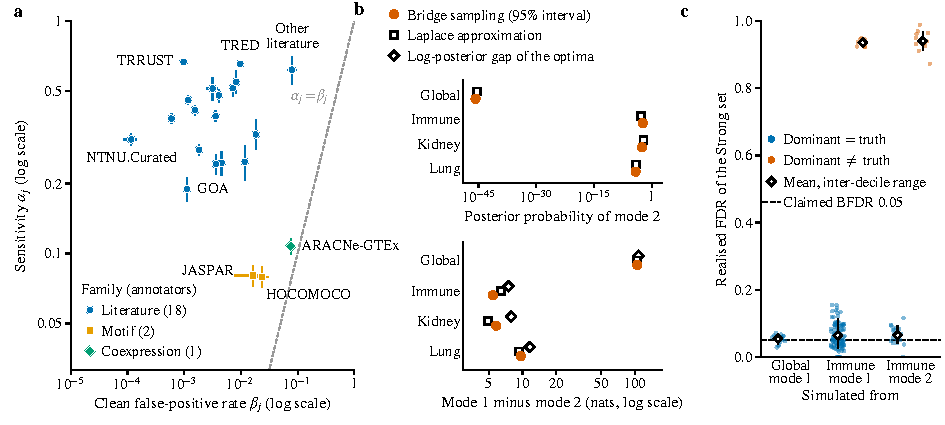
\includegraphics[width=\textwidth]{fig2_model.pdf}
  \caption{\textbf{Family-HB parameters and posterior modes.} (a) Annotator sensitivity $\alpha_j$ against clean false-positive rate $\beta_j$ (posterior means with 95\% credible intervals, global universe, NUTS) for the 21 held-in annotators (18 literature); the dashed diagonal is $\alpha_j=\beta_j$, which the parametrisation excludes. Sensitivities range from 0.08 to 0.67 and false-positive rates from 0.00012 to 0.079. (b) Mode 1 is the dominant posterior mode of each universe fit and mode 2 the second (in the global and immune fits, whose class weights are stored for both modes, mode 2 approximately exchanges the weights of the true class and the literature-burst class). Top: posterior probability of mode 2 by bridge sampling (filled; Monte Carlo 95\% interval) and by Laplace's method (open squares). Bottom: mode 1 minus mode 2 in log posterior mass (bridge sampling, filled; Laplace's method, open squares) and the log-posterior gap of the two optima (diamonds). Values and ranges in Table~\ref{tab:fit}. (c) Mode-selection simulation from the fitted model with the design-faithful simulator (data simulated at the parameters of the indicated mode with the real literature observation masks and the motif/coexpression masks rebuilt from the simulated literature reports, as in the evidence builder; the simulated data contain 59\% (immune) and 62\% (global) of the real number of motif- or coexpression-observed edges; refitted by multi-start MAP): realised false discovery rate of the Strong set for replicates whose dominant mode is or is not the truth mode (points: replicates; diamonds: mean with inter-decile range over replicates; dashed line: claimed BFDR 0.05); global universe, truth = mode 1: dominant mode is the truth mode in all 20 replicates, mean realised FDR 0.05; immune universe, truth = mode 1: dominant mode is the truth mode in 93 of 100 replicates, mean realised FDR 0.06 when it is and 0.94 when it is not; immune universe, truth = mode 2: dominant mode is the truth mode in 18 of 30 replicates, mean realised FDR 0.06 when it is and 0.94 when it is not. Sensitivity, probability that the dominant mode is the truth mode with every observation mask fixed at the real one: global universe 0.70, immune universe 0.68, immune universe (truth = mode 2) 0.77; with class weights that depend on the literature-mask stratum: global universe 1.00, immune universe 1.00, immune universe (truth = mode 2) 0.97 (Supplementary Table~\ref{tab:S-modes-sim}). The bridge-sampling estimates in (b) and panel (c) are post hoc (defined after the held-out data had been examined; no held-out data are used).}
  \label{fig:model}
\end{figure}


\paragraph{Which annotators carry information.}
Under the global fit the most diagnostic annotators, measured by the likelihood ratio of a report under the true class against the mixture of all non-true classes (post hoc summaries of the global NUTS fit), are SIGNOR (\nLrSignor{} [\nLrSignorLo{}, \nLrSignorHi{}]), TRRUST (\nLrTrrust{} [\nLrTrrustLo{}, \nLrTrrustHi{}]) and HTRIdb (\nLrHtridb{} [\nLrHtridbLo{}, \nLrHtridbHi{}]); motif and coexpression reports are only weakly diagnostic (Supplementary Table~\ref{tab:S-annotator-params}).
NTNU.Curated, which would look most diagnostic if only clean negatives were considered, ranks \nLrNtnuRank{} (\nLrNtnu{} [\nLrNtnuLo{}, \nLrNtnuHi{}]) because it reports burst edges more often than true edges ($\alpha/\gamma=\nAgNtnu{}$ [\nAgNtnuLo{}, \nAgNtnuHi{}]): about \nNtnuInExtriPct{}\% of its edges are also reported by the text-mining resource ExTRI.
The EM baseline, which assumes conditional independence, counts such co-reports as independent confirmation, and its Strong set is \nStrongRatioGlob{} times larger than that of Family-HB in the global universe (\nStrongEmGlob{} versus \nStrongHbGlob{} edges, posterior-mode credibilities).
In data simulated from the fitted Family-HB model (design-faithful simulator; \nRecNImm{} immune-design and \nRecNGlob{} global-design replicates) the EM Strong set has a realised false discovery rate of \nRecFdrEmMin{}--\nRecFdrEmMax{}, against \nRecFdrHbTruth{} for Family-HB when its fit selects the true mode; the immune value over all replicates, \nRecFdrHbImm{}, includes the \nRecNCompImm{} replicates whose fit selected the competing mode (Supplementary Table~\ref{tab:S-recovery}).
Because these data are generated with the dependence structure that Family-HB estimates, the comparison favours Family-HB by construction; it shows what ignoring the dependence costs if the dependence is as Family-HB estimates, not that the real data have this structure.

\paragraph{Label-free model checking.}
Without using any validation label, \nCvFolds{}-fold cross-validation with folds formed by TF prefers the burst models: the held-out log-likelihood per observed edge of the EM baseline is lower than that of Family-HB by \nCvEmGlob{} ($\pm$\nCvEmGlobSe{}) nats in the global universe and \nCvEmImm{} ($\pm$\nCvEmImmSe{}) in the immune universe, in all \nCvFoldsHbBetter{} folds of the two universes.
Posterior predictive checks reveal a misfit that all five estimators share: the probability that an edge is reported by at least one literature resource rises much faster with the number of literature resources that cover it than any model predicts (Supplementary Fig.~\ref{fig:S-ppc}; observed \nPpcObsOne{} versus predicted \nPpcRepOne{} for edges covered by one resource; observed \nPpcObsEight{} versus predicted \nPpcRepEight{} for edges covered by eight or more).
Well-studied gene pairs are covered by many resources and reported by many of them, a dependence on study intensity that none of the latent-class models represents.
This misfit is the first sign of the failure examined in \Cref{sec:res-heldout}.


\subsection{Family-HB is not more robust to annotator dropout than simpler estimators}\label{sec:res-robustness}

Removing one annotator at a time barely changes how any estimator ranks the \nRobNMethodsImm{} (immune) or \nRobNMethodsKidLung{} (kidney, lung) inference methods of the tissue universes (\Cref{tab:robustness}, \Cref{fig:robustness}).
Pooled over tissues and the \nRobNconf{} source-dropout configurations, the mean rank disagreement $D$ is \nRobDUnion{} for union, \nRobDVote{} for vote fraction, \nRobDEm{} for the EM baseline, \nRobDMaj{} for majority, \nRobDHb{} for Family-HB, \nRobDDep{} for the dependence-aware model, \nRobDSto{} for Stouffer, \nRobDFis{} for Fisher and \nRobDMf{} for the multifactor model.
Paired against EM over the same configurations (source-clustered, unadjusted 95\% intervals), every model with a burst class is less stable than EM: Family-HB slightly, by \nRobCtHbEm{} [\nRobCtHbEmLo{}, \nRobCtHbEmHi{}] (the interval only just excludes 0; \Cref{tab:robustness}), and, in post hoc contrasts with EM, the dependence-aware model by \nRobCtDepEm{} [\nRobCtDepEmLo{}, \nRobCtDepEmHi{}] and the multifactor model by \nRobCtMfEm{} [\nRobCtMfEmLo{}, \nRobCtMfEmHi{}].
Fisher, Stouffer and majority are also less stable than EM (post hoc; differences \nRobCtRuleEmMin{}--\nRobCtRuleEmMax{}), whereas union and vote fraction are not distinguishable from it.
% provenance: paper/r2/tables/tab_robustness.tex generated by src/r2/paper_assets on 2026-10-15 04:06 from data/r2/tables/
%   rob_method_ranking.csv (modified 2026-10-14 19:32): tissue == all_tissues & metric == f1 & subset in {all, no_fhb_mode_switch}; lineage: subset == excl_uninformative (configurations in which Family-HB is identified, the same for every estimator)
%   rob_estimator_contrasts.csv (modified 2026-10-14 19:32): scope == all_tissues & metric == D_f1 & reference == family_hb & protocol == source & subset in {all, no_fhb_mode_switch}
%   rob_edge_stability.csv (modified 2026-10-14 19:32): universe == global & protocol == source & subset == all
%   robustness.py.csv: NEAR_BEST (log-posterior distance counted as the same mode)
\begin{table}[tbp]
\centering
\small
\caption{Robustness to annotator dropout. (a) Rank disagreement $D$ of the tissue-method ranking (posterior-weighted $F_1$), three tissue universes pooled, with and without the configurations in which Family-HB switches posterior mode. (b) Edge-level stability in the global universe under single-source dropout (21 configurations): full-data sets against dropout sets.}
\label{tab:robustness}
{
\footnotesize
\setlength{\tabcolsep}{4pt}
\par\noindent\emph{(a) Method ranking, tissue universes}\par\smallskip
\begin{tabular}{@{}lcccccc@{}}
\toprule
 & \multicolumn{2}{c}{Source dropout (63)} & \multicolumn{2}{c}{Without mode switches (61)$^{\dagger}$} & Family (9) & Lineage (6)$^{\dagger}$ \\
\cmidrule(lr){2-3}\cmidrule(lr){4-5}
Estimator & $D$ & $\Delta D$ & $D$ & $\Delta D$ & $D$ & $D$ \\
\midrule
\multicolumn{7}{@{}l}{\emph{Latent-class estimators}} \\
EM baseline & \begin{tabular}[t]{@{}c@{}}0.008\\[-1pt]{\scriptsize [0.003, 0.015]}\end{tabular} & \begin{tabular}[t]{@{}c@{}}$-$0.008\\[-1pt]{\scriptsize [$-$0.017, $-$0.0001]}\end{tabular} & \begin{tabular}[t]{@{}c@{}}0.008\\[-1pt]{\scriptsize [0.003, 0.015]}\end{tabular} & \begin{tabular}[t]{@{}c@{}}$-$0.004\\[-1pt]{\scriptsize [$-$0.009, 0.001]}\end{tabular} & \begin{tabular}[t]{@{}c@{}}0.220\\[-1pt]{\scriptsize [0.000, 0.660]}\end{tabular} & \begin{tabular}[t]{@{}c@{}}0.065\\[-1pt]{\scriptsize [0.032, 0.098]}\end{tabular} \\
Dependence-aware & \begin{tabular}[t]{@{}c@{}}0.017\\[-1pt]{\scriptsize [0.009, 0.025]}\end{tabular} & \begin{tabular}[t]{@{}c@{}}0.000\\[-1pt]{\scriptsize [$-$0.009, 0.008]}\end{tabular} & \begin{tabular}[t]{@{}c@{}}0.016\\[-1pt]{\scriptsize [0.009, 0.025]}\end{tabular} & \begin{tabular}[t]{@{}c@{}}0.004\\[-1pt]{\scriptsize [$-$0.002, 0.010]}\end{tabular} & \begin{tabular}[t]{@{}c@{}}0.220\\[-1pt]{\scriptsize [0.000, 0.647]}\end{tabular} & \begin{tabular}[t]{@{}c@{}}0.153$^{b}$\\[-1pt]{\scriptsize [0.100, 0.206]}\end{tabular} \\
Multifactor & \begin{tabular}[t]{@{}c@{}}0.058\\[-1pt]{\scriptsize [0.039, 0.080]}\end{tabular} & \begin{tabular}[t]{@{}c@{}}0.041\\[-1pt]{\scriptsize [0.023, 0.059]}\end{tabular} & \begin{tabular}[t]{@{}c@{}}0.058\\[-1pt]{\scriptsize [0.038, 0.079]}\end{tabular} & \begin{tabular}[t]{@{}c@{}}0.046\\[-1pt]{\scriptsize [0.029, 0.065]}\end{tabular} & \begin{tabular}[t]{@{}c@{}}0.309\\[-1pt]{\scriptsize [0.061, 0.712]}\end{tabular} & \begin{tabular}[t]{@{}c@{}}0.176$^{b}$\\[-1pt]{\scriptsize [0.166, 0.186]}\end{tabular} \\
Family-regularized & \begin{tabular}[t]{@{}c@{}}0.009\\[-1pt]{\scriptsize [0.003, 0.015]}\end{tabular} & \begin{tabular}[t]{@{}c@{}}$-$0.008\\[-1pt]{\scriptsize [$-$0.017, 0.000]}\end{tabular} & \begin{tabular}[t]{@{}c@{}}0.009\\[-1pt]{\scriptsize [0.004, 0.015]}\end{tabular} & \begin{tabular}[t]{@{}c@{}}$-$0.004\\[-1pt]{\scriptsize [$-$0.009, 0.001]}\end{tabular} & \begin{tabular}[t]{@{}c@{}}0.218\\[-1pt]{\scriptsize [0.000, 0.654]}\end{tabular} & \begin{tabular}[t]{@{}c@{}}0.065\\[-1pt]{\scriptsize [0.032, 0.098]}\end{tabular} \\
Family-HB & \begin{tabular}[t]{@{}c@{}}0.017\\[-1pt]{\scriptsize [0.009, 0.025]}\end{tabular} & -- & \begin{tabular}[t]{@{}c@{}}0.012\\[-1pt]{\scriptsize [0.007, 0.017]}\end{tabular} & -- & \begin{tabular}[t]{@{}c@{}}0.227\\[-1pt]{\scriptsize [0.000, 0.449]}\end{tabular} & \begin{tabular}[t]{@{}c@{}}0.120$^{b}$\\[-1pt]{\scriptsize [0.090, 0.151]}\end{tabular} \\
\addlinespace[3pt]
\multicolumn{7}{@{}l}{\emph{Combination rules}} \\
Union & \begin{tabular}[t]{@{}c@{}}0.005\\[-1pt]{\scriptsize [0.002, 0.009]}\end{tabular} & \begin{tabular}[t]{@{}c@{}}$-$0.012\\[-1pt]{\scriptsize [$-$0.021, $-$0.003]}\end{tabular} & \begin{tabular}[t]{@{}c@{}}0.005\\[-1pt]{\scriptsize [0.002, 0.008]}\end{tabular} & \begin{tabular}[t]{@{}c@{}}$-$0.007\\[-1pt]{\scriptsize [$-$0.012, $-$0.003]}\end{tabular} & \begin{tabular}[t]{@{}c@{}}0.037\\[-1pt]{\scriptsize [0.000, 0.111]}\end{tabular} & \begin{tabular}[t]{@{}c@{}}0.035\\[-1pt]{\scriptsize [0.023, 0.048]}\end{tabular} \\
Majority ($\geq$2) & \begin{tabular}[t]{@{}c@{}}0.014\\[-1pt]{\scriptsize [0.008, 0.019]}\end{tabular} & \begin{tabular}[t]{@{}c@{}}$-$0.003\\[-1pt]{\scriptsize [$-$0.012, 0.004]}\end{tabular} & \begin{tabular}[t]{@{}c@{}}0.013\\[-1pt]{\scriptsize [0.008, 0.019]}\end{tabular} & \begin{tabular}[t]{@{}c@{}}0.001\\[-1pt]{\scriptsize [$-$0.004, 0.006]}\end{tabular} & \begin{tabular}[t]{@{}c@{}}0.073\\[-1pt]{\scriptsize [0.006, 0.195]}\end{tabular} & \begin{tabular}[t]{@{}c@{}}0.066\\[-1pt]{\scriptsize [0.047, 0.085]}\end{tabular} \\
Vote fraction & \begin{tabular}[t]{@{}c@{}}0.007\\[-1pt]{\scriptsize [0.003, 0.012]}\end{tabular} & \begin{tabular}[t]{@{}c@{}}$-$0.009\\[-1pt]{\scriptsize [$-$0.018, $-$0.002]}\end{tabular} & \begin{tabular}[t]{@{}c@{}}0.006\\[-1pt]{\scriptsize [0.003, 0.010]}\end{tabular} & \begin{tabular}[t]{@{}c@{}}$-$0.006\\[-1pt]{\scriptsize [$-$0.011, $-$0.002]}\end{tabular} & \begin{tabular}[t]{@{}c@{}}0.059\\[-1pt]{\scriptsize [0.000, 0.160]}\end{tabular} & \begin{tabular}[t]{@{}c@{}}0.051\\[-1pt]{\scriptsize [0.036, 0.065]}\end{tabular} \\
Fisher & \begin{tabular}[t]{@{}c@{}}0.022\\[-1pt]{\scriptsize [0.014, 0.032]}\end{tabular} & \begin{tabular}[t]{@{}c@{}}0.005\\[-1pt]{\scriptsize [$-$0.006, 0.016]}\end{tabular} & \begin{tabular}[t]{@{}c@{}}0.022\\[-1pt]{\scriptsize [0.013, 0.032]}\end{tabular} & \begin{tabular}[t]{@{}c@{}}0.010\\[-1pt]{\scriptsize [0.002, 0.019]}\end{tabular} & \begin{tabular}[t]{@{}c@{}}0.100\\[-1pt]{\scriptsize [0.019, 0.250]}\end{tabular} & \begin{tabular}[t]{@{}c@{}}0.078\\[-1pt]{\scriptsize [0.038, 0.117]}\end{tabular} \\
Stouffer & \begin{tabular}[t]{@{}c@{}}0.019\\[-1pt]{\scriptsize [0.011, 0.029]}\end{tabular} & \begin{tabular}[t]{@{}c@{}}0.003\\[-1pt]{\scriptsize [$-$0.006, 0.012]}\end{tabular} & \begin{tabular}[t]{@{}c@{}}0.019\\[-1pt]{\scriptsize [0.011, 0.030]}\end{tabular} & \begin{tabular}[t]{@{}c@{}}0.007\\[-1pt]{\scriptsize [0.000, 0.015]}\end{tabular} & \begin{tabular}[t]{@{}c@{}}0.081\\[-1pt]{\scriptsize [0.006, 0.225]}\end{tabular} & \begin{tabular}[t]{@{}c@{}}0.063\\[-1pt]{\scriptsize [0.028, 0.098]}\end{tabular} \\
\bottomrule
\end{tabular}
}
\par\medskip
{
\footnotesize
\setlength{\tabcolsep}{5pt}
\par\noindent\emph{(b) Edges, global universe}\par\smallskip
\begin{tabular}{@{}lrccc@{}}
\toprule
 & & \multicolumn{2}{c}{Jaccard index [95\% CI]} &  \\
\cmidrule(lr){3-4}
Estimator & $|S|$ & BFDR\,$\le$\,0.05 set & Size-matched$^{\dagger}$ & Spearman \\
\midrule
\multicolumn{5}{@{}l}{\emph{Latent-class estimators}} \\
EM baseline & 18{,}873 & 0.92 [0.85, 0.98] & 0.88 [0.80, 0.95] & 0.980 \\
Dependence-aware & 3{,}842 & 0.84 [0.74, 0.92] & 0.88 [0.81, 0.93] & 0.972 \\
Multifactor & 223 & 0.80 [0.69, 0.90] & 0.80 [0.71, 0.87] & 0.965 \\
Family-regularized & 18{,}873 & 0.92 [0.85, 0.98] & 0.88 [0.80, 0.95] & 0.980 \\
Family-HB & 4{,}064 & 0.85 [0.76, 0.92] & 0.87 [0.81, 0.92] & 0.979 \\
\addlinespace[3pt]
\multicolumn{5}{@{}l}{\emph{Combination rules}} \\
Union & 43{,}444 & 0.97 [0.94, 0.99] & 0.95 [0.91, 0.98] & 0.986 \\
Majority ($\geq$2) & 17{,}086 & 0.95 [0.90, 0.98] & 0.91 [0.85, 0.96] & 0.971 \\
Vote fraction & 4{,}992 & 0.92 [0.86, 0.96] & 0.90 [0.82, 0.96] & 0.986 \\
Fisher & 26{,}796 & 0.94 [0.90, 0.97] & 0.86 [0.80, 0.92] & 0.982 \\
Stouffer & 21{,}243 & 0.93 [0.88, 0.97] & 0.86 [0.80, 0.92] & 0.986 \\
\bottomrule
\end{tabular}
}
\par\smallskip
\begin{minipage}{\linewidth}\footnotesize
Lineage dropout$^{\dagger}$: the 6 configurations in which Family-HB is identified, for every estimator (the other 3 of 9 leave one modality family); Family-HB switches posterior mode in 4 of them. $^{b}$\,Includes dropout fits whose optimum was found only by the extended start search or the independent-seed check (post hoc).

$\Delta D$: paired difference to Family-HB (negative: more stable). Intervals: unadjusted 95\% bootstrap intervals over configurations clustered by the dropped source, family or lineage (one cluster across the three tissues$^{\dagger}$); family and lineage dropout (three families or lineages per tissue): descriptive. Mode switches$^{\dagger}$: in 2 of 63 source configurations (lung, SIGNOR and TRRUST dropped) the selected Family-HB dropout optimum is not the continuation of the full-data mode (warm-started fit more than $1.0\times 10^{-3}$ log-posterior units below it); the right-hand source columns drop them for every estimator, which conditions on the Family-HB fit and decomposes, but does not replace, the prespecified columns.

(b) $|S|$: size of the full-data posterior-mode BFDR\,$\le$\,0.05 set (for a 0/1 rule its positives, several times the Family-HB set, which favours the rules' Jaccard index); size-matched: top $n$ edges, $n$ the size of the Family-HB set; Spearman: scores of observed edges. One configuration per source, so the intervals are source-clustered; no Family-HB mode switch.

$^{\dagger}$\,Post hoc: defined after the held-out data had been examined.
\end{minipage}
\end{table}

% generated by src/r2/paper_assets (make_paper_assets.py figures); do not edit by hand
% provenance: fig3_robustness generated by src/r2/paper_assets on 2026-10-15 04:07 from data/r2/tables/
%   rob_method_ranking.csv (modified 2026-10-14 19:32): tissue = all_tissues, metric = f1, subset in {all, no_fhb_mode_switch (post hoc)}; lineage: subset = excl_uninformative (post hoc; the configurations in which Family-HB is identified, the same for every estimator); source-clustered intervals mean_D_cluster_lo/hi
%   rob_edge_stability.csv (modified 2026-10-14 19:32): protocol = source, subset = all; jaccard_bfdr_mean and jaccard_top_sizematched_mean (post hoc) with bootstrap intervals over configurations
%   rob_estimator_contrasts.csv (modified 2026-10-14 19:32): reference = family_hb, subset = all, scope = all_tissues (D_f1) or universe (jaccard_bfdr)
%   (constants): bfdr_strong from r2.common.PRESPECIFIED
\begin{figure}[tbp]
  \centering
  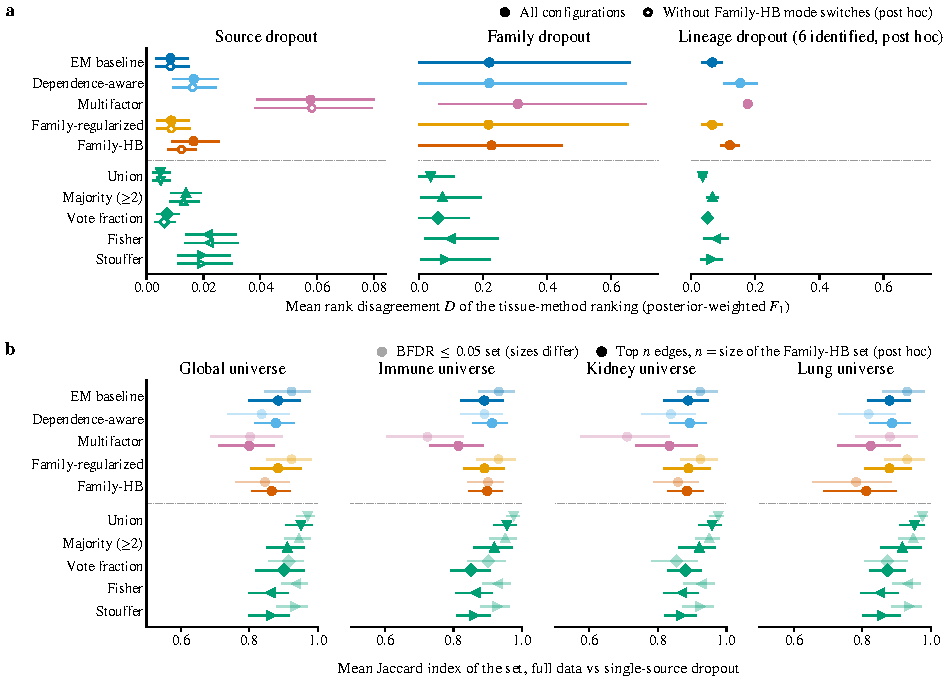
\includegraphics[width=\textwidth]{fig3_robustness.pdf}
  \caption{\textbf{Robustness to annotator dropout.} (a) Mean rank disagreement $D$ \eqref{eq:rankdisagreement} between the method ranking under the full-data credibility and under dropout of one source, one modality family or one integrator lineage, pooled over the three tissue universes (63 source, 9 family and 6 lineage configurations), with 95\% bootstrap intervals clustered by the dropped source, family or lineage (post hoc); family and lineage intervals are descriptive (at most three configurations per universe). Source dropout: Family-HB 0.017 [0.009, 0.025], EM 0.008 [0.003, 0.015], union 0.005 [0.002, 0.009]; open markers (post hoc): the 61 configurations left after removing the 2 in which Family-HB switches posterior mode (lung, SIGNOR and TRRUST dropped), Family-HB 0.012 [0.007, 0.017], EM 0.008 [0.003, 0.015]. Lineage dropout (post hoc): the 6 configurations in which Family-HB is identified, for every estimator (dropping the DoRothEA lineage leaves one modality family, so Family-HB is not identified in 3 of the 9 lineage configurations; post hoc identification rule): Family-HB 0.120 [0.090, 0.151], EM 0.065 [0.032, 0.098]; Family-HB switches posterior mode in 4 of them. (b) Mean Jaccard index between the full-data and the single-source dropout sets (faded markers: BFDR $\leq 0.05$ set; filled markers (post hoc): top $n$ edges, $n$ the size of the Family-HB set), with 95\% bootstrap intervals over the dropout configurations (one per source). For a 0/1 rule the BFDR set is its set of positives, several times larger than the Family-HB set (global universe: Family-HB 4{,}064, EM 18{,}873, union 43{,}444 edges), which inflates its Jaccard index. Global universe, BFDR set: Family-HB 0.85 [0.76, 0.92], EM 0.92 [0.85, 0.98], union 0.97 [0.94, 0.99]; size-matched: Family-HB 0.87 [0.81, 0.92], EM 0.88 [0.80, 0.95], union 0.95 [0.91, 0.98]. The Family-HB values of the lung universe include the source configurations in which Family-HB switches posterior mode (lung, SIGNOR and TRRUST dropped; size-matched Family-HB lung 0.81 [0.69, 0.90]).}
  \label{fig:robustness}
\end{figure}

The family-regularized model, which adds only the hierarchical prior to EM, gives essentially the same results as EM here, on held-out data and in the hub simulations (\Cref{tab:robustness,tab:heldout}, Supplementary Table~\ref{tab:S-simhub}): hierarchical pooling alone has no measurable effect in these data, and the differences between Family-HB and EM come from its burst classes.

About half of the Family-HB--EM difference (\nRobGapSharePct{}\%) comes from \nRobNswitch{} configurations, lung with SIGNOR or with TRRUST dropped, which are the two with the largest disagreement for Family-HB (\nRobDSwitchMin{} and \nRobDSwitchMax{}, against at most \nRobDNoSwitchMax{} in the other configurations); in both, the dropout optimum is a different posterior mode from the continuation of the full-data mode.
Without these configurations (\nRobNconfNs{} configurations; a post hoc decomposition that conditions on an outcome of the Family-HB fit and does not replace the full comparison), Family-HB is not distinguishable from EM ($D$ \nRobDHbNs{} against \nRobDEmNs{}; difference \nRobCtHbEmNs{} [\nRobCtHbEmNsLo{}, \nRobCtHbEmNsHi{}]), but the dependence-aware model, which does not switch mode under source dropout, is still less stable than EM ($D$ \nRobDDepNs{}; difference \nRobCtDepEmNs{} [\nRobCtDepEmNsLo{}, \nRobCtDepEmNsHi{}]).
On $D$, union and vote fraction remain more stable than Family-HB (differences \nRobCtUnionNs{} [\nRobCtUnionNsLo{}, \nRobCtUnionNsHi{}] and \nRobCtVoteNs{} [\nRobCtVoteNsLo{}, \nRobCtVoteNsHi{}]), and Fisher and Stouffer are not more stable than Family-HB.

At the edge level, credibility rankings change little under any estimator (mean Spearman correlation between full-data and dropout credibilities \nRobSpMin{}--\nRobSpMax{} in the global universe).
Sets selected at a fixed BFDR are more stable in the global universe for EM (Jaccard \nRobJacBfdrEm{}) and union (\nRobJacBfdrUnion{}) than for Family-HB (\nRobJacBfdrHb{}), but these sets differ in size.
At equal set size (post hoc), pooled over tissues, Family-HB (\nRobSmHb{}) is not distinguishable from EM (\nRobSmEm{}; difference \nRobSmCtHbEm{} [\nRobSmCtHbEmLo{}, \nRobSmCtHbEmHi{}]); only union (\nRobSmUnion{}; \nRobSmCtUnionEm{} [\nRobSmCtUnionEmLo{}, \nRobSmCtUnionEmHi{}]) and majority (\nRobSmMaj{}; \nRobSmCtMajEm{} [\nRobSmCtMajEmLo{}, \nRobSmCtMajEmHi{}]) are more stable than EM, and the dependence-aware model (\nRobSmDep{}) is more stable than Family-HB (\nRobSmCtDepHb{} [\nRobSmCtDepHbLo{}, \nRobSmCtDepHbHi{}]) but not distinguishable from EM.
Without the \nRobNswitch{} mode-switch configurations, Family-HB and EM are not distinguishable at equal size either (\nRobSmHbNs{} and \nRobSmEmNs{}).
In the global universe, where Family-HB never switches mode under source dropout, EM is more stable at equal size in \nRobSmGlobNEm{} of \nRobSmGlobN{} configurations, although the mean difference (Family-HB minus EM \nRobSmCtHbEmGlob{} [\nRobSmCtHbEmGlobLo{}, \nRobSmCtHbEmGlobHi{}]) is not distinguishable from zero.

Removing all annotators that reached us through one integrator separates the estimators more (\nRobLinN{} identified tissue configurations; post hoc, descriptive): mean disagreement \nRobLinHb{} for Family-HB against \nRobLinEm{} for EM and \nRobLinUnion{} for union.
The separation lies in the \nRobLinNSw{} configurations in which Family-HB switches mode (\nRobLinHbSw{} against \nRobLinEmSw{} for EM); in the other \nRobLinNs{} the order reverses (\nRobLinHbNs{} against \nRobLinEmNs{}).
With so few configurations, with the removal of the multi-integrator annotators in all three tissues among the switches, and with several lineage-dropout optima of the latent-class models reached by few random starts, this comparison is only indicative.

\emph{Interpretation.} Models with a burst class have a small true class (posterior weight \nWtPctMin{}--\nWtPctMax{}\% of edges), so their top-ranked sets depend on fewer reports and move more when one report source disappears; Family-HB can in addition switch between its two modes.
None of these summaries shows Family-HB more stable than EM: in these data, modelling dependence buys no robustness.
Stability is in any case not accuracy: a rule that ignored the evidence would be perfectly stable.


\subsection{On held-out data Family-HB does not outperform simple combination rules}\label{sec:res-heldout}

The central test of a credibility estimator is whether it ranks edges that are supported by held-out evidence above edges that are not.
In the global universe, against \nHoNevalEncMio{} million ENCODE-evaluable, \nHoNevalEnetMio{} million ENETS2-evaluable and \nHoNevalPertMio{} million perturbation-evaluable edges, Family-HB (posterior-mode credibilities, as for every latent-class estimator in these comparisons) has an AP lift of \nApHbEnc{} [\nApHbEncLo{}, \nApHbEncHi{}] on ENCODE, \nApHbEnet{} [\nApHbEnetLo{}, \nApHbEnetHi{}] on ENETS2 and \nApHbPert{} [\nApHbPertLo{}, \nApHbPertHi{}] on the pooled perturbation reference (\Cref{tab:heldout}, \Cref{fig:heldout}a).
The EM baseline is close (\nApEmEnc{}, \nApEmEnet{} and \nApEmPert{}): slightly better on ENCODE (paired difference \nPairEmEnc{} [\nPairEmEncLo{}, \nPairEmEncHi{}], Holm $p=\nPairEmEncP{}$) and not distinguishable on ENETS2 and perturbation data.
Fisher's method is better on both ChIP references (\nApFiEnc{} and \nApFiEnet{}; paired differences \nPairFiEnc{} and \nPairFiEnet{} in the primary comparison family, Holm-adjusted $p=\nPairFiChipP{}$ for both, the smallest attainable value), and so is Stouffer's (\nApStEnc{} and \nApStEnet{}).
On ENETS2 Family-HB exceeds the held-in DoRothEA levels (difference \nPairDorEnet{} [\nPairDorEnetLo{}, \nPairDorEnetHi{}], Holm $p=\nPairDorEnetP{}$).
On perturbation data no score is far from random: Family-HB \nApHbPert{}, Fisher \nApFiPert{}, vote count \nApVcPert{}, DoRothEA \nApDorPert{}, CollecTRI \nApColPert{}.
The composition-adjusted AP lift, the AP lift divided by its expectation when edges are ranked at random within TFs (post hoc, descriptive), shows that most of the pooled perturbation difference between Family-HB and the simple rules reflects which TFs carry many positives, not ranking within TFs: that expectation is \nCompNullHb{} for Family-HB, which ranks edges of TFs with few positives first, against \nCompNullCmpMin{}--\nCompNullCmpMax{} for the five non-EM comparators.
After adjustment Family-HB (\nAdjHb{} [\nAdjHbLo{}, \nAdjHbHi{}]) is \nPairAdjFi{} below mid-$p$ Fisher (Holm $p=\nPairAdjFiP{}$ over the six comparators) and \nPairAdjVcCol{} below the vote count and CollecTRI (Holm $p=\nPairAdjVcColP{}$, the smallest attainable value).
Against a variant of Fisher's method without the mid-$p$ rule, which ties covered-but-unreported edges with uncovered ones, the gap is \nPairAdjFiSec{} [\nPairAdjFiSecLo{}, \nPairAdjFiSecHi{}] (post hoc), so the small gap to mid-$p$ Fisher is a property of that rule.
Within TFs Family-HB ranks at or below random: its within-TF AUROC is \nAucHbPert{} [\nAucHbPertLo{}, \nAucHbPertHi{}], and its AP is below that of every within-TF permutation of the labels (permutation $p=\nPermHbPert{}$), although the TF-bootstrap interval of its composition-adjusted AP lift includes 1, because the bootstrap generalises over TFs while the permutation test conditions on them.
Moving its uncovered edges last (a post hoc mechanism check, below) restores a random within-TF order (\nAucUlPert{}) but leaves the global composition-adjusted AP lift unchanged (\nAdjUlPert{}).
% provenance: paper/r2/tables/tab_heldout.tex generated by src/r2/paper_assets on 2026-10-15 04:06 from data/r2/tables/
%   heldout_estimators.csv (modified 2026-10-14 20:06): universe == global & eval_subset == all_evaluable; columns ap_lift, ap_lift_comp_adj (+ _lo/_hi), within_tf_auroc, enr_at_500 (+ _lo/_hi), strat_enr_at_500
%   heldout_paired.csv (modified 2026-10-14 20:06): universe == global & eval_subset == all_evaluable & {metric == ap_lift & analysis_role == confirmatory; metric == ap_lift_comp_adj & confirmatory_comparator}
\begin{table}[tbp]
\centering
\small
\renewcommand{\arraystretch}{0.93}
\caption{Held-out evaluation in the global universe (all evaluable edges): AP lift and composition-adjusted AP lift (95\% TF-cluster bootstrap intervals; Holm $p$ of Family-HB (MAP) against each comparator of the primary comparison family), within-TF AUROC, and enrichment of the top 500 edges, unstratified and stratified.}
\label{tab:heldout}
{
\footnotesize
\setlength{\tabcolsep}{2.4pt}
\begin{tabular}{@{}lccccccc@{}}
\toprule
 & \multicolumn{2}{c}{AP lift} & \multicolumn{2}{c}{Composition-adjusted AP lift$^{\dagger}$} & Within-TF & \multicolumn{2}{c}{Enr@500} \\
\cmidrule(lr){2-3}\cmidrule(lr){4-5}\cmidrule(lr){7-8}
Score & [95\% CI] & Holm $p$$^{\dagger}$ & [95\% CI] & Holm $p$$^{\dagger}$ & AUROC & [95\% CI] & Strat. \\
\midrule
\multicolumn{8}{@{}l}{\emph{ENCODE TFBS: 1{,}037{,}801 evaluable edges, 395{,}408 positives, 107 TFs}} \\
Family-HB (NUTS) & 0.96 [0.94, 0.98] & -- & 0.97 [0.96, 0.97] & -- & 0.481 & 1.63 [1.35, 1.93] & 1.33 \\
Family-HB (MAP) & 0.96 [0.94, 0.98] & -- & 0.97 [0.96, 0.97] & -- & 0.481 & 1.62 [1.34, 1.92] & 1.32 \\
EM baseline & 0.96 [0.95, 0.98] & $7.8\times 10^{-3}$ & 0.97 [0.97, 0.98] & $\leq$$1.2\times 10^{-3}$ & 0.489 & 1.35 [1.19, 1.55] & 1.33 \\
Dependence-aware & 0.96 [0.95, 0.98] & -- & 0.97 [0.96, 0.98] & -- & 0.485 & 1.68 [1.37, 1.94] & 1.39 \\
Multifactor & 0.96 [0.94, 0.97] & -- & 0.97 [0.96, 0.97] & -- & 0.482 & 1.87 [1.57, 2.12] & 1.45 \\
Family-regularized & 0.96 [0.95, 0.98] & -- & 0.97 [0.97, 0.98] & -- & 0.489 & 1.35 [1.20, 1.55] & 1.33 \\
\addlinespace[2pt]
Union & 1.01 [1.00, 1.01] & -- & 1.00 [1.00, 1.01] & -- & 0.505 & 1.31 [1.12, 1.50] & 1.13 \\
Majority ($\geq$2) & 1.00 [1.00, 1.01] & -- & 1.00 [1.00, 1.00] & -- & 0.504 & 1.38 [1.18, 1.57] & 1.20 \\
Vote count & 1.01 [1.00, 1.01] & $\leq$$1.2\times 10^{-3}$ & 1.01 [1.00, 1.01] & $\leq$$1.2\times 10^{-3}$ & 0.505 & 1.59 [1.38, 1.81] & 1.46 \\
Fisher & 1.07 [1.05, 1.08] & $\leq$$1.2\times 10^{-3}$ & 1.06 [1.05, 1.07] & $\leq$$1.2\times 10^{-3}$ & 0.547 & 1.46 [1.26, 1.66] & 1.50 \\
Stouffer & 1.04 [1.03, 1.06] & $\leq$$1.2\times 10^{-3}$ & 1.04 [1.04, 1.05] & $\leq$$1.2\times 10^{-3}$ & 0.534 & 1.47 [1.28, 1.67] & 1.53 \\
\addlinespace[2pt]
DoRothEA level & 1.01 [1.00, 1.01] & $\leq$$1.2\times 10^{-3}$ & 1.00 [1.00, 1.01] & $\leq$$1.2\times 10^{-3}$ & 0.504 & 1.58 [1.23, 1.91] & 1.18 \\
CollecTRI & 1.00 [1.00, 1.01] & $\leq$$1.2\times 10^{-3}$ & 1.00 [1.00, 1.01] & $\leq$$1.2\times 10^{-3}$ & 0.504 & 1.23 [0.94, 1.60] & 1.48 \\
\addlinespace[2pt]
Random & 1.00 [1.00, 1.00] & -- & 1.00 [1.00, 1.00] & -- & 0.500 & 1.01 [0.91, 1.11] & 1.01 \\
\addlinespace[3pt]
\multicolumn{8}{@{}l}{\emph{ENETS2: 755{,}798 evaluable edges, 10{,}826 positives, 82 TFs}} \\
Family-HB (NUTS) & 1.58 [1.31, 2.00] & -- & 1.58 [1.30, 1.98] & -- & 0.522 & 12.29 [8.76, 17.29] & 6.66 \\
Family-HB (MAP) & 1.59 [1.31, 2.00] & -- & 1.58 [1.30, 1.98] & -- & 0.522 & 12.57 [8.78, 17.49] & 6.79 \\
EM baseline & 1.49 [1.26, 1.83] & 0.29 & 1.49 [1.26, 1.81] & 0.25 & 0.529 & 10.89 [7.12, 15.43] & 7.09 \\
Dependence-aware & 1.59 [1.31, 2.02] & -- & 1.58 [1.31, 2.01] & -- & 0.525 & 12.71 [8.47, 18.05] & 7.07 \\
Multifactor & 1.70 [1.40, 2.15] & -- & 1.70 [1.40, 2.16] & -- & 0.516 & 18.85 [13.59, 24.15] & 12.28 \\
Family-regularized & 1.50 [1.26, 1.83] & -- & 1.49 [1.26, 1.81] & -- & 0.529 & 10.94 [7.13, 15.34] & 7.05 \\
\addlinespace[2pt]
Union & 1.33 [1.19, 1.53] & -- & 1.31 [1.18, 1.51] & -- & 0.533 & 4.67 [3.67, 6.06] & 2.82 \\
Majority ($\geq$2) & 1.30 [1.17, 1.49] & -- & 1.29 [1.16, 1.48] & -- & 0.523 & 6.45 [4.90, 8.57] & 3.90 \\
Vote count & 1.60 [1.34, 1.97] & 0.70 & 1.58 [1.33, 1.94] & 0.82 & 0.533 & 14.28 [10.30, 18.92] & 8.39 \\
Fisher & 1.80 [1.48, 2.27] & $\leq$$1.2\times 10^{-3}$ & 1.74 [1.45, 2.17] & $1.0\times 10^{-2}$ & 0.537 & 13.96 [9.36, 19.14] & 9.34 \\
Stouffer & 1.80 [1.47, 2.28] & $2.0\times 10^{-3}$ & 1.76 [1.45, 2.21] & $5.0\times 10^{-3}$ & 0.527 & 14.24 [9.77, 19.45] & 9.70 \\
\addlinespace[2pt]
DoRothEA level & 1.37 [1.20, 1.62] & $2.4\times 10^{-3}$ & 1.36 [1.20, 1.60] & $3.6\times 10^{-3}$ & 0.523 & 8.35 [5.92, 11.90] & 4.10 \\
CollecTRI & 1.43 [1.25, 1.70] & 0.16 & 1.42 [1.25, 1.69] & 0.13 & 0.528 & 10.97 [7.58, 14.05] & 6.59 \\
\addlinespace[2pt]
Random & 1.01 [0.99, 1.03] & -- & 1.00 [0.98, 1.03] & -- & 0.503 & 1.12 [0.41, 2.01] & 1.11 \\
\addlinespace[3pt]
\multicolumn{8}{@{}l}{\emph{Pooled perturbation: 484{,}173 evaluable edges, 46{,}945 positives, 110 TFs}} \\
Family-HB (NUTS) & 0.94 [0.90, 0.98] & -- & 0.99 [0.97, 1.01] & -- & 0.478 & 2.10 [1.39, 3.55] & 1.53 \\
Family-HB (MAP) & 0.94 [0.90, 0.98] & -- & 0.99 [0.97, 1.01] & -- & 0.478 & 2.10 [1.38, 3.56] & 1.53 \\
EM baseline & 0.94 [0.90, 0.98] & 0.69 & 0.99 [0.97, 1.01] & 0.42 & 0.479 & 2.37 [1.42, 3.49] & 1.47 \\
Dependence-aware & 0.94 [0.90, 0.98] & -- & 0.99 [0.97, 1.01] & -- & 0.478 & 2.10 [1.44, 3.51] & 1.55 \\
Multifactor & 0.93 [0.89, 0.98] & -- & 0.98 [0.97, 1.00] & -- & 0.473 & 2.08 [1.24, 2.93] & 1.77 \\
Family-regularized & 0.94 [0.90, 0.98] & -- & 0.99 [0.97, 1.01] & -- & 0.479 & 2.33 [1.42, 3.48] & 1.45 \\
\addlinespace[2pt]
Union & 1.01 [1.00, 1.03] & -- & 1.01 [1.00, 1.02] & -- & 0.507 & 1.66 [1.16, 2.38] & 1.25 \\
Majority ($\geq$2) & 1.01 [1.00, 1.03] & -- & 1.01 [1.00, 1.02] & -- & 0.507 & 2.07 [1.38, 3.11] & 1.41 \\
Vote count & 1.02 [1.01, 1.05] & $3.7\times 10^{-2}$ & 1.02 [1.01, 1.04] & $\leq$$1.2\times 10^{-3}$ & 0.507 & 2.71 [1.63, 4.02] & 1.59 \\
Fisher & 1.01 [0.98, 1.06] & $5.8\times 10^{-2}$ & 0.99 [0.97, 1.01] & 0.56 & 0.497 & 2.46 [1.57, 3.61] & 1.52 \\
Stouffer & 1.02 [0.99, 1.06] & $3.8\times 10^{-2}$ & 1.00 [0.99, 1.02] & $6.7\times 10^{-2}$ & 0.502 & 2.56 [1.62, 3.61] & 1.55 \\
\addlinespace[2pt]
DoRothEA level & 1.01 [1.00, 1.02] & $3.8\times 10^{-2}$ & 1.01 [1.00, 1.02] & $8.8\times 10^{-3}$ & 0.505 & 1.74 [1.11, 3.42] & 1.43 \\
CollecTRI & 1.02 [1.01, 1.04] & $3.7\times 10^{-2}$ & 1.02 [1.01, 1.03] & $\leq$$1.2\times 10^{-3}$ & 0.507 & 2.73 [1.49, 4.28] & 1.68 \\
\addlinespace[2pt]
Random & 0.99 [0.99, 1.00] & -- & 0.99 [0.98, 1.00] & -- & 0.508 & 0.83 [0.65, 1.02] & 0.85 \\
\bottomrule
\end{tabular}
}
\par\smallskip
\begin{minipage}{\linewidth}\footnotesize
Holm $p$: Family-HB (MAP) minus comparator, paired TF-cluster bootstrap (10{,}000 resamples), Holm over the 6 comparators of the primary comparison family (post hoc) of each reference ($\leq$: resampling floor; --: not tested; the NUTS fit was not tested). Composition-adjusted AP lift: AP over its exact expectation under permutation of the labels within TFs (1: no ranking signal within TFs); its paired tests are descriptive.

All lifts and enrichments equal 1, within-TF AUROC 0.5, for a random ranking. Enr@500: positives among the 500 highest-ranked edges over the base-rate expectation (the metric of the paired Enr@500 contrasts); Strat.: within TF $\times$ target-degree strata. All scores and references: Supplementary Tables~\ref{tab:S-heldout-chip}--\ref{tab:S-heldout-pert-enr}.

$^{\dagger}$\,Post hoc: defined after the held-out data had been examined.
\end{minipage}
\end{table}

% generated by src/r2/paper_assets (make_paper_assets.py figures); do not edit by hand
% provenance: fig4_heldout generated by src/r2/paper_assets on 2026-10-15 04:07 from data/r2/tables/
%   heldout_estimators.csv (modified 2026-10-14 20:06): universe = global, eval_subset = all_evaluable, reference in {encode, enets2, pert_pooled}; score in the plotted list
%   heldout_evidence_status.csv (modified 2026-10-14 20:08): reference in {encode, enets2, pert_pooled}
%   obs_heldout_status.csv (modified 2026-10-14 20:37): universe = global, reference = encode, status in {unobserved, observed_neg}: mean_cred_em (EM credibility by evidence status)
%   (constants): LOW_SUPPORT_TFS, LOW_SUPPORT_POS from r2.heldout_eval
\begin{figure}[tbp]
  \centering
  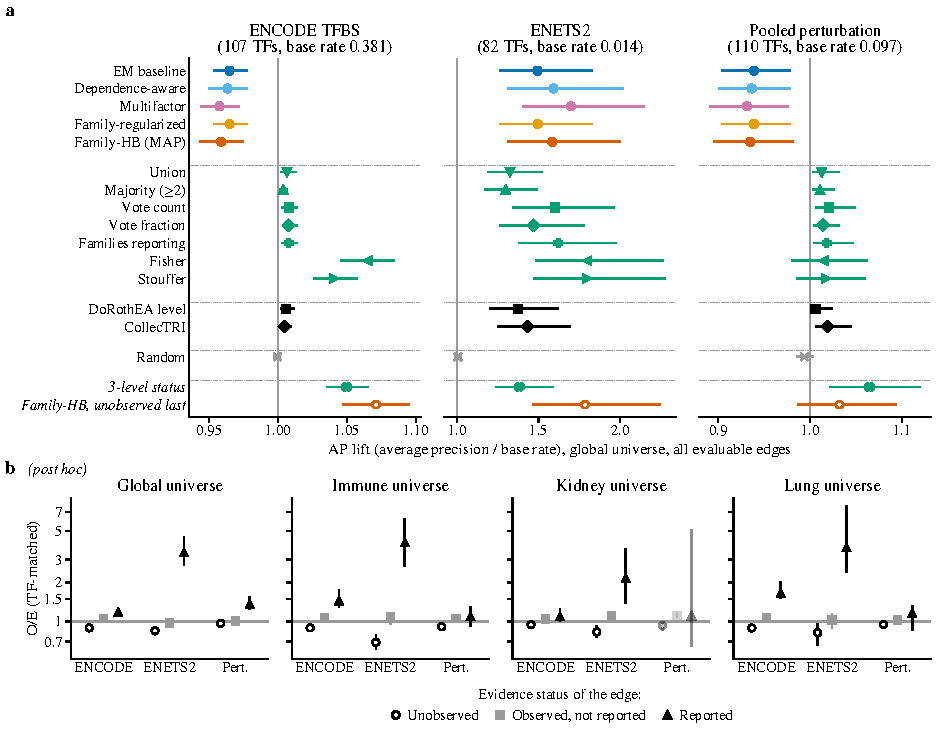
\includegraphics[width=\textwidth]{fig4_heldout.pdf}
  \caption{\textbf{Held-out evaluation in the global universe.} (a) AP lift of every score on all evaluable edges, with 95\% TF-bootstrap intervals; the vertical line marks a random ranking. Open italic rows are post hoc mechanism scores (the 3-level evidence status and Family-HB with unobserved edges ranked last); Family-HB (MAP) is the posterior-mode fit used in the paired tests. Family-HB: ENCODE 0.96 [0.94, 0.98], ENETS2 1.59 [1.31, 2.00], pooled perturbation 0.94 [0.90, 0.98]; Fisher: 1.07 [1.05, 1.08], 1.80 [1.48, 2.27], 1.01 [0.98, 1.06]; EM: 0.96 [0.95, 0.98], 1.49 [1.26, 1.83], 0.94 [0.90, 0.98]. (b) Positives among unobserved, observed but unreported, and reported edges relative to the TF-matched expectation (95\% TF-bootstrap intervals; faded: fewer than 10 TFs with positives or fewer than 20 positives); the whole panel is post hoc. Global universe, unobserved edges: ENCODE 0.89 [0.88, 0.91], ENETS2 0.85 [0.78, 0.90], pooled perturbation 0.97 [0.95, 0.98]; observed negatives 1.05 [1.04, 1.05] (ENCODE). Unobserved edges are depleted of positives in every universe (O/E 0.69 to 0.95 in the tissue universes), whereas the missing-at-random latent-class estimators give them a higher mean credibility than observed negatives (ENCODE-evaluable edges: Family-HB 0.0031 vs 0.00099; EM 0.0068 vs 0.0021): coverage is informative (inference: not missing at random).}
  \label{fig:heldout}
\end{figure}


\paragraph{Why: coverage is not missing at random.}
Over the full universe every latent-class estimator ranks worse than random within TFs on ENCODE and on pooled perturbation data in the global universe (within-TF AUROC \nAucLcmMin{}--\nAucLcmMax{}, every interval below 0.5).
The reason is visible in a post hoc breakdown by the evidence status of edges (\Cref{tab:status}, \Cref{fig:heldout}b).
Relative to the TF-matched expectation, edges that no annotator covers are depleted of held-out positives (observed over expected \nStUnobsEnc{} [\nStUnobsEncLo{}, \nStUnobsEncHi{}] for ENCODE, \nStUnobsEnet{} [\nStUnobsEnetLo{}, \nStUnobsEnetHi{}] for ENETS2, \nStUnobsPert{} [\nStUnobsPertLo{}, \nStUnobsPertHi{}] for perturbation), edges covered but not reported are at expectation (\nStObsnegEnc{}, \nStObsnegEnet{}, \nStObsnegPert{}), and reported edges are enriched (\nStRepEnc{}, \nStRepEnet{}, \nStRepPert{}).
Under the missing-at-random assumption, however, an uncovered edge keeps the prior credibility $w_{\mathrm{T}}$, whereas a covered edge that no annotator reports is pushed below it: Family-HB gives uncovered edges a mean credibility of \nStCredUnobs{} and covered-but-unreported edges \nStCredObsneg{}, the reverse of the held-out ordering.
Fisher and Stouffer avoid the problem only because they give uncovered edges the lowest score.
% provenance: paper/r2/tables/tab_status.tex generated by src/r2/paper_assets on 2026-10-15 04:06 from data/r2/tables/
%   heldout_evidence_status.csv (modified 2026-10-14 20:08): reference in {encode, enets2, pert_pooled}
\begin{table}[tbp]
\centering
\small
\caption{Held-out positive rate by evidence status (post hoc analysis$^{\dagger}$): observed over TF-matched expected positives (O/E, 95\% TF-cluster bootstrap interval) and mean Family-HB credibility $\bar c$ of evaluable edges that no annotator observes, that are observed but not reported, or that carry at least one report.}
\label{tab:status}
\begin{tabular}{@{}lcccccc@{}}
\toprule
Universe & \multicolumn{2}{c}{Unobserved} & \multicolumn{2}{c}{Observed, not reported} & \multicolumn{2}{c}{Reported} \\
\cmidrule(lr){2-3}\cmidrule(lr){4-5}\cmidrule(lr){6-7}
 & O/E & $\bar c$ & O/E & $\bar c$ & O/E & $\bar c$ \\
\midrule
\multicolumn{7}{@{}l}{\emph{ENCODE TFBS}} \\
Global & \begin{tabular}[t]{@{}c@{}}0.89\\[-1pt]{\scriptsize [0.88, 0.91]}\end{tabular} & 0.0031 & \begin{tabular}[t]{@{}c@{}}1.05\\[-1pt]{\scriptsize [1.04, 1.05]}\end{tabular} & $9.9\times 10^{-4}$ & \begin{tabular}[t]{@{}c@{}}1.17\\[-1pt]{\scriptsize [1.11, 1.24]}\end{tabular} & 0.24 \\
Immune & \begin{tabular}[t]{@{}c@{}}0.89\\[-1pt]{\scriptsize [0.87, 0.91]}\end{tabular} & 0.0063 & \begin{tabular}[t]{@{}c@{}}1.07\\[-1pt]{\scriptsize [1.06, 1.09]}\end{tabular} & 0.0015 & \begin{tabular}[t]{@{}c@{}}1.44\\[-1pt]{\scriptsize [1.28, 1.78]}\end{tabular} & 0.26 \\
Kidney & \begin{tabular}[t]{@{}c@{}}0.95\\[-1pt]{\scriptsize [0.93, 0.95]}\end{tabular} & 0.0063 & \begin{tabular}[t]{@{}c@{}}1.05\\[-1pt]{\scriptsize [1.04, 1.06]}\end{tabular} & 0.0015 & \begin{tabular}[t]{@{}c@{}}1.09\\[-1pt]{\scriptsize [1.00, 1.26]}\end{tabular} & 0.26 \\
Lung & \begin{tabular}[t]{@{}c@{}}0.89\\[-1pt]{\scriptsize [0.87, 0.91]}\end{tabular} & 0.0047 & \begin{tabular}[t]{@{}c@{}}1.07\\[-1pt]{\scriptsize [1.05, 1.08]}\end{tabular} & $9.8\times 10^{-4}$ & \begin{tabular}[t]{@{}c@{}}1.65\\[-1pt]{\scriptsize [1.49, 2.02]}\end{tabular} & 0.27 \\
\addlinespace[3pt]
\multicolumn{7}{@{}l}{\emph{ENETS2}} \\
Global & \begin{tabular}[t]{@{}c@{}}0.85\\[-1pt]{\scriptsize [0.78, 0.90]}\end{tabular} & 0.0031 & \begin{tabular}[t]{@{}c@{}}0.98\\[-1pt]{\scriptsize [0.95, 1.01]}\end{tabular} & $9.9\times 10^{-4}$ & \begin{tabular}[t]{@{}c@{}}3.41\\[-1pt]{\scriptsize [2.70, 4.53]}\end{tabular} & 0.25 \\
Immune & \begin{tabular}[t]{@{}c@{}}0.69\\[-1pt]{\scriptsize [0.61, 0.79]}\end{tabular} & 0.0063 & \begin{tabular}[t]{@{}c@{}}1.09\\[-1pt]{\scriptsize [0.95, 1.18]}\end{tabular} & 0.0015 & \begin{tabular}[t]{@{}c@{}}4.05\\[-1pt]{\scriptsize [2.66, 6.21]}\end{tabular} & 0.26 \\
Kidney & \begin{tabular}[t]{@{}c@{}}0.83\\[-1pt]{\scriptsize [0.75, 0.93]}\end{tabular} & 0.0063 & \begin{tabular}[t]{@{}c@{}}1.10\\[-1pt]{\scriptsize [1.01, 1.17]}\end{tabular} & 0.0015 & \begin{tabular}[t]{@{}c@{}}2.15\\[-1pt]{\scriptsize [1.38, 3.63]}\end{tabular} & 0.28 \\
Lung & \begin{tabular}[t]{@{}c@{}}0.82\\[-1pt]{\scriptsize [0.66, 0.96]}\end{tabular} & 0.0047 & \begin{tabular}[t]{@{}c@{}}1.03\\[-1pt]{\scriptsize [0.89, 1.15]}\end{tabular} & $9.7\times 10^{-4}$ & \begin{tabular}[t]{@{}c@{}}3.73\\[-1pt]{\scriptsize [2.39, 7.83]}\end{tabular} & 0.29 \\
\addlinespace[3pt]
\multicolumn{7}{@{}l}{\emph{Pooled perturbation}} \\
Global & \begin{tabular}[t]{@{}c@{}}0.97\\[-1pt]{\scriptsize [0.95, 0.98]}\end{tabular} & 0.0031 & \begin{tabular}[t]{@{}c@{}}1.01\\[-1pt]{\scriptsize [1.00, 1.02]}\end{tabular} & 0.0011 & \begin{tabular}[t]{@{}c@{}}1.36\\[-1pt]{\scriptsize [1.24, 1.56]}\end{tabular} & 0.24 \\
Immune & \begin{tabular}[t]{@{}c@{}}0.91\\[-1pt]{\scriptsize [0.85, 0.95]}\end{tabular} & 0.0063 & \begin{tabular}[t]{@{}c@{}}1.06\\[-1pt]{\scriptsize [1.03, 1.11]}\end{tabular} & 0.0016 & \begin{tabular}[t]{@{}c@{}}1.09\\[-1pt]{\scriptsize [0.92, 1.31]}\end{tabular} & 0.28 \\
Kidney$^{*}$ & \begin{tabular}[t]{@{}c@{}}0.93\\[-1pt]{\scriptsize [0.86, 0.97]}\end{tabular} & 0.0063 & \begin{tabular}[t]{@{}c@{}}1.11\\[-1pt]{\scriptsize [1.07, 1.17]}\end{tabular} & 0.0018 & \begin{tabular}[t]{@{}c@{}}1.10\\[-1pt]{\scriptsize [0.64, 5.09]}\end{tabular} & 0.30 \\
Lung & \begin{tabular}[t]{@{}c@{}}0.95\\[-1pt]{\scriptsize [0.91, 0.98]}\end{tabular} & 0.0047 & \begin{tabular}[t]{@{}c@{}}1.03\\[-1pt]{\scriptsize [1.01, 1.06]}\end{tabular} & $9.2\times 10^{-4}$ & \begin{tabular}[t]{@{}c@{}}1.16\\[-1pt]{\scriptsize [0.86, 1.34]}\end{tabular} & 0.33 \\
\bottomrule
\end{tabular}
\par\smallskip
\begin{minipage}{\linewidth}\footnotesize
$^{*}$\,At least one status group has low support (few positives or TFs).

O/E = 1: positives occur at the rate expected from the TF's own positive rate. $\bar c$: mean posterior-mode credibility of the group.

$^{\dagger}$\,Post hoc: defined after the held-out data had been examined.
\end{minipage}
\end{table}

A post hoc check confirms the mechanism: a label-free score that merely orders uncovered below covered-unreported below reported edges reaches AP lifts of \nApStatusEnc{}, \nApStatusEnet{} and \nApStatusPert{}, and Family-HB with uncovered edges moved to the bottom reaches \nApUlEnc{}, \nApUlEnet{} and \nApUlPert{}, matching Fisher on the ChIP references.
Where the deficit lies depends on the reference and the universe.
On ENCODE it lies within TFs in both metrics (composition-adjusted AP lift \nAdjHbEnc{} against \nAdjFiEnc{} for Fisher; within-TF AUROC \nAucHbEnc{} [\nAucHbEncLo{}, \nAucHbEncHi{}]); on ENETS2 the within-TF deficit relative to mid-$p$ Fisher and Stouffer lies in AP only (within-TF AUROC difference to Fisher \nPairAucFiEnet{} [\nPairAucFiEnetLo{}, \nPairAucFiEnetHi{}]), whereas against EM the within-TF AUROC of Family-HB is slightly lower (\nPairAucEmEnet{} [\nPairAucEmEnetLo{}, \nPairAucEmEnetHi{}], Holm-adjusted bootstrap $p\le\nPairAucEmEnetP{}$, the resampling floor; descriptive).
On pooled perturbation data in the global universe most of the deficit is between-TF composition, although placing uncovered edges last still lifts the within-TF AUROC to random (above).
In the tissue universes, whose perturbation evidence comes from \nTfsPosTisMin{}--\nTfsPosTisMax{} TFs with positives, Family-HB has within-TF perturbation deficits (composition-adjusted AP lift \nAdjHbTisPertMin{}--\nAdjHbTisPertMax{}) that disappear when its uncovered edges are placed last (\nAdjUlTisPertMin{}--\nAdjUlTisPertMax{}), as on ChIP, and within-TF AUROC moves the same way. With so few TFs these comparisons are fragile: bootstrap intervals over so few clusters tend to be too narrow, percentile and normal-approximation bootstrap tests disagree for several of the tissue contrasts, and the coverage of the paired intervals was not checked by simulation.

\paragraph{The head of the ranking.}
The highest-credibility edges do carry held-out support: the \nEvalK{} top-ranked evaluable edges of Family-HB are enriched \nEnrHbEnc{}-fold [\nEnrHbEncLo{}, \nEnrHbEncHi{}] for ENCODE binding, \nEnrHbEnet{}-fold [\nEnrHbEnetLo{}, \nEnrHbEnetHi{}] for ENETS2 and \nEnrHbPert{}-fold [\nEnrHbPertLo{}, \nEnrHbPertHi{}] for perturbation positives, and \nSenrHbEnc{}-, \nSenrHbEnet{}- and \nSenrHbPert{}-fold after stratification by TF and target degree.
Restricted to edges with at least one held-in report, Family-HB is neither the best nor the worst estimator.
In the tissue universes, which contain \nChipTfsTisMin{}--\nChipTfsTisMax{} ChIP-assayed TFs each, Family-HB is below every non-EM comparator on ENCODE (differences \nTisEncDMin{} to \nTisEncDMax{}).
Expression-based network inference sets a sensible bar there, and Family-HB does not reach it.
The predicted sets (\nTopK{} targets per TF) of GRNBoost2 and of absolute Pearson correlation have a higher TF-matched ENCODE enrichment than the predicted set of Family-HB (posterior-mean credibility of the tissue fit) in every tissue: \nPsGbEncImm{} and \nPsPeEncImm{} against \nPsHbEncImm{} in immune, \nPsGbEncKid{} and \nPsPeEncKid{} against \nPsHbEncKid{} in kidney, and \nPsGbEncLung{} and \nPsPeEncLung{} against \nPsHbEncLung{} in lung (post hoc comparison of point estimates; Supplementary Table~\ref{tab:S-fm-heldout}).
On ENETS2 the same holds in immune (\nPsGbEnetImm{} and \nPsPeEnetImm{} against \nPsHbEnetImm{}) and kidney (\nPsGbEnetKid{} and \nPsPeEnetKid{} against \nPsHbEnetKid{}), and in kidney the Family-HB set is not above a random one (ENCODE \nPsHbEncKid{} against \nPsRandEncKid{}, ENETS2 \nPsHbEnetKid{} against \nPsRandEnetKid{}).
This is the coverage failure again: a tissue universe has only \nCtxRepPerTfMin{} to \nCtxRepPerTfMax{} reported edges per TF on average, so most of the \nTopK{} predicted targets of Family-HB are edges without any report, among which uncovered edges are ranked above covered but unreported ones (\Cref{tab:status}). Consistent with this, in a post hoc check the deficit shrinks for predicted sets of \nTopKSensLo{} targets per TF, which contain fewer unreported edges (ENCODE enrichment \nPsHbEncLoKMin{}--\nPsHbEncLoKMax{}; Supplementary Table~\ref{tab:S-fm-sens}).

\emph{Implication.} Fusing references with a latent-class model gives a defensible ranking of the edges the references actually speak to, but not of the universe as a whole. Any use of credibility over a candidate universe must treat uncovered pairs explicitly, which is what claim tiers built on reported edges do (\Cref{sec:res-governance}).


\subsection{Modelling coverage as informative does not repair the ranking}\label{sec:res-obs}

The extension of \Cref{sec:obsmodel}, which lets coverage by literature resources depend on the latent class, was fitted to EM and Family-HB in all universes (Supplementary Tables~\ref{tab:S-obs-fit}--\ref{tab:S-obs-heldout} and Fig.~\ref{fig:S-obs}).
It fails as a generative model.
The observation term contributes \nObsShare{}\% of the joint log-likelihood, and the latent class becomes an attribute of the target gene: \nObsVar{}\% of the variance of the credibility lies between target genes, against \nObsVarHb{}\% for Family-HB.
This happens because a resource's coverage of a pair is the gene's presence in the resource, repeated over every TF the resource covers.
The two models also choose opposite labellings: Family-HB with informative observation assigns the true class to rarely covered genes (class weight \nObsWtHbObs{}), EM with informative observation to frequently covered ones (\nObsWtEmObs{}); each model's label-swapped optimum is the other model's best.
Neither improves the prediction of reports in cross-validation.
On held-out data the Family-HB variant stays below random (ENCODE AP lift \nObsApHbObs{}), and the EM variant is above random (\nObsApEmObs{} [\nObsApEmObsLo{}, \nObsApEmObsHi{}]) but below the label-free status score (\nObsApStatus{}) and Fisher (\nObsApFisher{}); after stratification by TF and target degree its top \nEvalK{} edges carry essentially no enrichment (\nObsSenrEmObs{}), so it acts as a gene-popularity score.
Down-weighting the replicated observation term by the number of eligible TFs removes the degeneracy but returns credibilities nearly identical to Family-HB (Spearman \nObsTfwSp{}) and does not repair the ranking.
In the hub-bias simulation of \Cref{sec:inference} (post hoc), all \nObsSimN{} Family-HB fits with informative observation inflate the true class to \nObsSimWtAllPctMin{}--\nObsSimWtAllPctMax{}\% of the edges (scenario medians \nObsSimWtPctMin{}--\nObsSimWtPctMax{}\%, against a true share of about \nObsSimTruePct{}\%), so the failure is a property of the model rather than of these data.
\emph{Implication:} coverage is informative, but at the level of genes and TFs, not of individual edges, and an edge-level selection model cannot capture it; a gene-level coverage model is a natural next step.

\subsection{Context-matched gains in raw precision are prevalence effects}\label{sec:res-universe}

The perturbation positive rate is higher in every tissue-context universe than in the global universe, so raw precision can be higher there without any better ranking; read naively, such a gain looks like a benefit of matching the candidate universe to the biological context.
\Cref{eq:decomp} separates the two sources (\Cref{tab:decomp}, \Cref{fig:universe}).
In the immune universe the pooled perturbation positive rate is \nUniBaseImm{} against \nUniBaseGlob{} globally, a ratio of \nUniBr{}; the ratio of raw precision among the \nEvalK{} top-ranked edges is \nUniRaw{} [\nUniRawLo{}, \nUniRawHi{}], so the enrichment ratio is \nUniEnr{} [\nUniEnrLo{}, \nUniEnrHi{}]: the context ranking is \emph{less} enriched than the global one, and the whole raw gain is prevalence.
Random sub-universes of the global universe with the context's size and exactly its number of positives give a median precision of \nUniNull{} [\nUniNullLo{}, \nUniNullHi{}] against \nUniCtx{} in the context; \nUniSurvEdge{}\% of the raw gap survives an edge-level null and \nUniSurvBlock{}\% a null that samples whole TF blocks (post hoc; two-sided $p=\nUniPEdge{}$ and \nUniPBlock{}), and for best $F_1$ almost none of it survives (\nUniFOneSurv{}\%).
% provenance: paper/r2/tables/tab_decomp.tex generated by src/r2/paper_assets on 2026-10-15 04:06 from data/r2/tables/
%   heldout_universe_decomposition.csv (modified 2026-10-14 20:08): metric == p_at_500 & credibility == global_fit
%   heldout_downsampling_null.csv (modified 2026-10-14 20:08): metric == p_at_500 & credibility == global_fit & null in {prevalence_matched, tf_block_matched}
\begin{table}[tbp]
\centering
\small
\setlength{\tabcolsep}{4pt}
\caption{Universe-aware decomposition of the context--global difference in raw precision of the top 500 edges (global-fit Family-HB credibility): raw ratio = base-rate ratio $\times$ enrichment ratio, and comparison with prevalence-matched random sub-universes of the global universe drawn edge by edge or as whole TF blocks.}
\label{tab:decomp}
\begin{tabular}{@{}lccccccccc@{}}
\toprule
 & \multicolumn{2}{c}{Base rate} & \multicolumn{3}{c}{P@500} & \multicolumn{2}{c}{Edge null} & \multicolumn{2}{c}{TF-block null$^{\dagger}$} \\
\cmidrule(lr){2-3}\cmidrule(lr){4-6}\cmidrule(lr){7-8}\cmidrule(lr){9-10}
Tissue & Context & Ratio & Context & Raw ratio & Enrichment ratio & Median & Surviving & Median & Surviving \\
\midrule
\multicolumn{10}{@{}l}{\emph{ENCODE TFBS (global universe: P@500 = 0.62, base rate 0.38)}} \\
Immune & 0.24 & 0.62 & 0.41 & \begin{tabular}[t]{@{}c@{}}0.67\\[-1pt]{\scriptsize [0.49, 0.90]}\end{tabular} & \begin{tabular}[t]{@{}c@{}}1.08\\[-1pt]{\scriptsize [0.84, 1.40]}\end{tabular} & \begin{tabular}[t]{@{}c@{}}0.35\\[-1pt]{\scriptsize [0.31, 0.39]}\end{tabular} & $-$0.33 & \begin{tabular}[t]{@{}c@{}}0.32\\[-1pt]{\scriptsize [0.20, 0.49]}\end{tabular} & $-$0.48 \\
Kidney & 0.36 & 0.95 & 0.43 & \begin{tabular}[t]{@{}c@{}}0.69\\[-1pt]{\scriptsize [0.53, 0.88]}\end{tabular} & \begin{tabular}[t]{@{}c@{}}0.72\\[-1pt]{\scriptsize [0.58, 0.92]}\end{tabular} & \begin{tabular}[t]{@{}c@{}}0.48\\[-1pt]{\scriptsize [0.43, 0.52]}\end{tabular} & 0.26 & \begin{tabular}[t]{@{}c@{}}0.43\\[-1pt]{\scriptsize [0.32, 0.59]}\end{tabular} & 0.03 \\
Lung & 0.20 & 0.52 & 0.40 & \begin{tabular}[t]{@{}c@{}}0.65\\[-1pt]{\scriptsize [0.43, 0.87]}\end{tabular} & \begin{tabular}[t]{@{}c@{}}1.26\\[-1pt]{\scriptsize [0.95, 1.59]}\end{tabular} & \begin{tabular}[t]{@{}c@{}}0.28\\[-1pt]{\scriptsize [0.24, 0.32]}\end{tabular} & $-$0.55 & \begin{tabular}[t]{@{}c@{}}0.25\\[-1pt]{\scriptsize [0.17, 0.40]}\end{tabular} & $-$0.69 \\
\addlinespace[3pt]
\multicolumn{10}{@{}l}{\emph{Pooled perturbation (global universe: P@500 = 0.20, base rate 0.10)}} \\
Immune & 0.25 & 2.57 & 0.26 & \begin{tabular}[t]{@{}c@{}}1.28\\[-1pt]{\scriptsize [0.63, 2.51]}\end{tabular} & \begin{tabular}[t]{@{}c@{}}0.50\\[-1pt]{\scriptsize [0.30, 0.80]}\end{tabular} & \begin{tabular}[t]{@{}c@{}}0.25\\[-1pt]{\scriptsize [0.22, 0.27]}\end{tabular} & 0.27 & \begin{tabular}[t]{@{}c@{}}0.25\\[-1pt]{\scriptsize [0.22, 0.32]}\end{tabular} & 0.12 \\
Kidney & 0.15 & 1.55 & 0.14 & \begin{tabular}[t]{@{}c@{}}0.70\\[-1pt]{\scriptsize [0.28, 1.41]}\end{tabular} & \begin{tabular}[t]{@{}c@{}}0.45\\[-1pt]{\scriptsize [0.26, 0.73]}\end{tabular} & \begin{tabular}[t]{@{}c@{}}0.15\\[-1pt]{\scriptsize [0.14, 0.17]}\end{tabular} & 0.19 & \begin{tabular}[t]{@{}c@{}}0.15\\[-1pt]{\scriptsize [0.12, 0.20]}\end{tabular} & 0.19 \\
Lung & 0.29 & 3.04 & 0.29 & \begin{tabular}[t]{@{}c@{}}1.43\\[-1pt]{\scriptsize [0.73, 2.57]}\end{tabular} & \begin{tabular}[t]{@{}c@{}}0.47\\[-1pt]{\scriptsize [0.28, 0.73]}\end{tabular} & \begin{tabular}[t]{@{}c@{}}0.29\\[-1pt]{\scriptsize [0.27, 0.31]}\end{tabular} & 0.02 & \begin{tabular}[t]{@{}c@{}}0.30\\[-1pt]{\scriptsize [0.27, 0.35]}\end{tabular} & $-$0.13 \\
\bottomrule
\end{tabular}
\par\smallskip
\begin{minipage}{\linewidth}\footnotesize
Ratios are context over global. Null: median and 95\% interval of P@500 over random sub-universes with the context's number of evaluable edges and exactly its number of positives, drawn as edges or as whole TF blocks matched to the context's per-TF sizes and positive counts. Surviving: fraction of the context--global gap not reproduced by the null, (context $-$ null median)/(context $-$ global); negative values mean that the context value exceeds its null although raw precision falls. The edge-level null ignores the clustering of edges within TFs and is anti-conservative; the TF-block null keeps it.

Intervals: TF-cluster bootstrap of the context and the global set drawn independently (conservative when the sets share TFs)$^{\dagger}$.

$^{\dagger}$\,Post hoc: defined after the held-out data had been examined.
\end{minipage}
\end{table}

% generated by src/r2/paper_assets (make_paper_assets.py figures); do not edit by hand
% provenance: fig5_universe generated by src/r2/paper_assets on 2026-10-15 04:07 from data/r2/tables/
%   heldout_universe_decomposition.csv (modified 2026-10-14 20:08): metric = p_at_500
%   heldout_downsampling_null.csv (modified 2026-10-14 20:08): metric = p_at_500, null in {prevalence_matched (edge sampling), tf_block_matched (whole TF blocks; post hoc)}
%   (constants): FIG5_K (one of r2.common.PRESPECIFIED['eval_k'])
\begin{figure}[tbp]
  \centering
  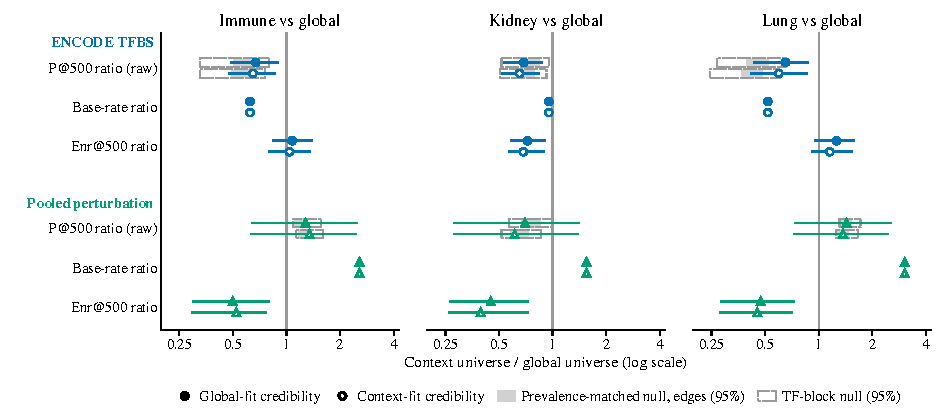
\includegraphics[width=\textwidth]{fig5_universe.pdf}
  \caption{\textbf{Universe-aware decomposition of context-versus-global differences.} For each tissue and reference, the ratio of precision among the 500 highest-credibility evaluable edges in the context universe to that in the global universe (raw P@500 ratio) is the product of the base-rate ratio and the Enr@500 ratio \eqref{eq:decomp}; 95\% intervals (post hoc) combine independent TF bootstraps of the two universes. Filled markers: Family-HB credibility from the global fit; open markers: from the context fit. Grey bars: central 95\% of the raw ratio under the prevalence-matched null (1{,}000 random sub-universes of the global universe with the context's numbers of evaluable edges and positives, sampled as edges); dashed boxes: the same null sampled as whole TF blocks matched to the context's per-TF sizes (post hoc), which keeps the within-TF dependence. Pooled perturbation, global-fit credibility: immune: raw 1.28 = base rate 2.57 $\times$ enrichment 0.50 [0.30, 0.80]; kidney: raw 0.70 = base rate 1.55 $\times$ enrichment 0.45 [0.26, 0.73]; lung: raw 1.43 = base rate 3.04 $\times$ enrichment 0.47 [0.28, 0.73]. On ENCODE the raw immune ratio is 0.67 although the enrichment ratio is 1.08, because the context base rate is lower (0.24 vs 0.38); the context P@500 (0.41) lies outside the edge-level null distribution (median 0.35, two-sided empirical $p=4.0\times 10^{-3}$, post hoc) and inside the TF-block null distribution (median 0.32, $p=0.21$); the edge-level null ignores the clustering of edges within TFs and is anti-conservative.}
  \label{fig:universe}
\end{figure}

In kidney and lung the context ranking is also less enriched than the global one (enrichment ratios \nUniEnrKid{} and \nUniEnrLung{}); raw precision is nominally higher in lung (ratio \nUniRawLung{} [\nUniRawLungLo{}, \nUniRawLungHi{}]) and lower in kidney (\nUniRawKid{} [\nUniRawKidLo{}, \nUniRawKidHi{}]), where the weaker context ranking outweighs the higher prevalence; as in immune, the raw-precision interval includes 1 in lung.
On ENCODE the context and global rankings are not distinguishable after matching TF blocks (post hoc; two-sided $p$ \nUniEncPImm{}, \nUniEncPKid{} and \nUniEncPLung{} for immune, kidney and lung).
\emph{Implication:} precision-type metrics cannot be compared across candidate universes, however the universes are chosen; differences must be reported on a prevalence-free scale and against a matched null.


\subsection{Label-free claim tiers in foundation-model contexts}\label{sec:res-governance}

\paragraph{Tier sizes.}
Dual-universe governance promotes \nGovPromImm{} edges in the immune universe (Strong \nGovStrongImm{}, Moderate \nGovModImm{}), \nGovPromKid{} in kidney and \nGovPromLung{} in lung, \nGovShareMin{}--\nGovShareMax{}\% of each context universe (\Cref{tab:governance}); posterior draws give intervals of \nGovPromImmLo{}--\nGovPromImmHi{}, \nGovPromKidLo{}--\nGovPromKidHi{} and \nGovPromLungLo{}--\nGovPromLungHi{} promoted edges.
The BFDR of the promoted set under the context fit is \nGovBfdrPromMin{}--\nGovBfdrPromMax{}, but that of the Moderate tier alone is \nGovBfdrModMin{}--\nGovBfdrModMax{} under the context fit and \nGovBfdrModGlobMin{}--\nGovBfdrModGlobMax{} under the global fit: between one in three and two in five Moderate claims are expected to be false, and Moderate claims should be read as hypotheses.
The two fits agree moderately on the level of an edge (linearly weighted $\kappa$ \nGovKappaMin{}--\nGovKappaMax{} among edges at least Moderate under either).
% provenance: paper/r2/tables/tab_governance.tex generated by src/r2/paper_assets on 2026-10-15 04:06 from data/r2/tables/
%   gov_tiers.csv (modified 2026-10-14 20:11): scope == dual
%   gov_consistency.csv (modified 2026-10-14 20:11): credibility == nuts & scope in {all_edges, either_ge_moderate}
%   gov_tier_validation.csv (modified 2026-10-14 20:11): tissues: scope == dual & tier == Promoted; global: scope == global_fit & tier in {Strong, Moderate, Promoted}
\begin{table}[tbp]
\centering
\small
\caption{Claim governance. Dual-universe tiers in the tissue-context universes (95\% interval over posterior draws), their posterior expected FDR under the global and the context fit, agreement of the two fits, and held-out enrichment of promoted edges after TF matching (O/E, 95\% TF-cluster bootstrap interval). Global universe: single-fit tiers.}
\label{tab:governance}
\begin{tabular}{@{}lcccc@{}}
\toprule
 & Immune & Kidney & Lung & Global \\
\midrule
\multicolumn{5}{@{}l}{\emph{Tier size (edges)}} \\
Strong & \begin{tabular}[t]{@{}c@{}}297\\[-1pt]{\scriptsize [275, 309]}\end{tabular} & \begin{tabular}[t]{@{}c@{}}149\\[-1pt]{\scriptsize [128, 160]}\end{tabular} & \begin{tabular}[t]{@{}c@{}}204\\[-1pt]{\scriptsize [170, 230]}\end{tabular} & 4{,}060 \\
Moderate & \begin{tabular}[t]{@{}c@{}}196\\[-1pt]{\scriptsize [178, 205]}\end{tabular} & \begin{tabular}[t]{@{}c@{}}127\\[-1pt]{\scriptsize [107, 130]}\end{tabular} & \begin{tabular}[t]{@{}c@{}}208\\[-1pt]{\scriptsize [174, 211]}\end{tabular} & 3{,}274 \\
Conditional & \begin{tabular}[t]{@{}c@{}}73\\[-1pt]{\scriptsize [61, 141]}\end{tabular} & \begin{tabular}[t]{@{}c@{}}56\\[-1pt]{\scriptsize [51, 126]}\end{tabular} & \begin{tabular}[t]{@{}c@{}}63\\[-1pt]{\scriptsize [50, 177]}\end{tabular} & -- \\
Promoted (Strong $\cup$ Moderate) & \begin{tabular}[t]{@{}c@{}}493\\[-1pt]{\scriptsize [456, 512]}\end{tabular} & \begin{tabular}[t]{@{}c@{}}276\\[-1pt]{\scriptsize [237, 289]}\end{tabular} & \begin{tabular}[t]{@{}c@{}}412\\[-1pt]{\scriptsize [344, 434]}\end{tabular} & 7{,}334$^{\dagger}$ \\
\addlinespace[3pt]
\multicolumn{5}{@{}l}{\emph{Posterior expected FDR (global fit / context fit)}} \\
Strong & 0.048 / 0.036 & 0.046 / 0.034 & 0.044 / 0.041 & -- \\
Promoted & 0.190 / 0.159 & 0.195 / 0.157 & 0.191 / 0.167 & -- \\
\addlinespace[3pt]
\multicolumn{5}{@{}l}{\emph{Agreement of global and context fit (linearly weighted $\kappa$)}} \\
All edges & 0.93 & 0.90 & 0.92 & -- \\
Edges $\geq$ Moderate in either fit & 0.67 & 0.58 & 0.64 & -- \\
\addlinespace[3pt]
\multicolumn{5}{@{}l}{\emph{Held-out O/E of promoted edges, TF-matched}} \\
ENCODE TFBS & \begin{tabular}[t]{@{}c@{}}1.67\\[-1pt]{\scriptsize [1.35, 2.38]}\end{tabular} & \begin{tabular}[t]{@{}c@{}}1.24\\[-1pt]{\scriptsize [1.03, 1.81]}\end{tabular} & \begin{tabular}[t]{@{}c@{}}2.27\\[-1pt]{\scriptsize [1.78, 3.37]}\end{tabular} & \begin{tabular}[t]{@{}c@{}}1.26$^{\dagger}$\\[-1pt]{\scriptsize [1.16, 1.43]}\end{tabular} \\
ENETS2 & \begin{tabular}[t]{@{}c@{}}5.95\\[-1pt]{\scriptsize [3.39, 9.05]}\end{tabular} & \begin{tabular}[t]{@{}c@{}}3.66\\[-1pt]{\scriptsize [1.30, 7.65]}\end{tabular} & \begin{tabular}[t]{@{}c@{}}6.74\\[-1pt]{\scriptsize [4.12, 13.83]}\end{tabular} & \begin{tabular}[t]{@{}c@{}}5.29$^{\dagger}$\\[-1pt]{\scriptsize [3.86, 8.13]}\end{tabular} \\
Pooled perturbation & \begin{tabular}[t]{@{}c@{}}1.20\\[-1pt]{\scriptsize [0.82, 1.64]}\end{tabular} & \begin{tabular}[t]{@{}c@{}}0.66$^{*}$\\[-1pt]{\scriptsize [0.00, 1.00]}\end{tabular} & \begin{tabular}[t]{@{}c@{}}1.29$^{*}$\\[-1pt]{\scriptsize [1.13, 1.57]}\end{tabular} & \begin{tabular}[t]{@{}c@{}}1.71$^{\dagger}$\\[-1pt]{\scriptsize [1.45, 2.16]}\end{tabular} \\
\bottomrule
\end{tabular}
\par\smallskip
\begin{minipage}{\linewidth}\footnotesize
$^{*}$\,Few TF clusters among the evaluable promoted edges; interval unreliable.

Single-fit levels: Strong, the largest prefix of whole tie blocks with posterior expected FDR $\leq$ 0.05; Moderate, the largest prefix with $\leq$ 0.20, minus Strong. Dual tiers: Strong if Strong under both fits (the intersection of the two single-fit Strong sets); Moderate if at least Moderate under both, not Strong; Conditional if at least Moderate under exactly one fit. Tiers use posterior-mean credibilities. The global universe has a single fit, so it has no Conditional tier and no cross-universe agreement (--).

$^{\dagger}$\,Post hoc: defined after the held-out data had been examined.
\end{minipage}
\end{table}


\paragraph{Held-out validation.}
After matching on TF, promoted edges are enriched for ENCODE binding (observed over expected \nGovOeEncImm{} [\nGovOeEncImmLo{}, \nGovOeEncImmHi{}] in immune, \nGovOeEncKid{} [\nGovOeEncKidLo{}, \nGovOeEncKidHi{}] in kidney, \nGovOeEncLung{} [\nGovOeEncLungLo{}, \nGovOeEncLungHi{}] in lung) and for ENETS2 edges (\nGovOeEnetImm{}, \nGovOeEnetKid{} and \nGovOeEnetLung{}), and the enrichment declines from the promoted tiers to Exploratory, which holds almost all edges and lies slightly below expectation (ENCODE \nGovExplEncMin{}--\nGovExplEncMax{}, ENETS2 \nGovExplEnetMin{}--\nGovExplEnetMax{}). The decline is not strict tier by tier: in immune the Moderate tier is as enriched for ENCODE binding as the Strong tier, and in kidney none of the \nGovModEnetKidNeval{} ENETS2-evaluable Moderate edges is an ENETS2 positive (\Cref{fig:governance}b).
A one-sided Mantel trend test across the four tiers (a screen, because it treats the edges of a stratum as exchangeable; \Cref{sec:governance}), stratified by TF and target degree, gives Holm-adjusted $p\le \nGovTrendChipMax{}$ for every tissue and ChIP reference; stratified by TF alone it gives $p\le\nGovTrendTfOtherMax{}$ except for kidney, where $p=\nGovTrendTfKidEnc{}$ on ENCODE and \nGovTrendTfKidStrict{} on ENCODE-strict, so the kidney gradient depends on adjusting for target degree.
In the global universe the gradient also appears in perturbation data (Strong \nGovGlobPertStrong{} [\nGovGlobPertStrongLo{}, \nGovGlobPertStrongHi{}], Moderate \nGovGlobPertMod{} [\nGovGlobPertModLo{}, \nGovGlobPertModHi{}], below Moderate \nGovGlobPertBelow{}), and on ENETS2 it is steep (\nGovGlobEnetStrong{}, \nGovGlobEnetMod{}, \nGovGlobEnetBelow{}).
In the tissue universes the perturbation evidence is thin: promoted O/E \nGovOePertImm{} [\nGovOePertImmLo{}, \nGovOePertImmHi{}] in immune (\nGovPertNtfImm{} evaluable TFs), \nGovOePertKid{} [\nGovOePertKidLo{}, \nGovOePertKidHi{}] in kidney and \nGovOePertLung{} [\nGovOePertLungLo{}, \nGovOePertLungHi{}] in lung, the last two from \nGovPertNtfKid{} and \nGovPertNtfLung{} evaluable TFs, too few for reliable bootstrap intervals.
Only the immune result is informative, and it does not support the tiers: its interval excludes the global-universe effect of \nGovPertGlobOe{}, which the immune design had power \nGovPertPowImm{} to detect (a post hoc power calculation from the design margins).
Low power is therefore not the explanation there; the cohorts are K562 and THP-1 cells, unrelated to the tissues, and single TFs dominate the evaluable edges (SPI1 holds \nGovPertTopTfPctMin{}--\nGovPertTopTfPctMax{}\% of them in immune and lung).
Part of the ChIP enrichment passes through literature records that themselves rest on ChIP evidence.
% generated by src/r2/paper_assets (make_paper_assets.py figures); do not edit by hand
% provenance: fig6_governance generated by src/r2/paper_assets on 2026-10-15 04:07 from data/r2/tables/
%   gov_tiers.csv (modified 2026-10-14 20:11): scope = dual, tier in {Strong, Moderate, Conditional}; draw interval columns
%   gov_tier_validation.csv (modified 2026-10-14 20:11): universe = global (scope global_fit) or tissues (scope dual); tier in {Strong, Moderate, Conditional}; reference in {encode, enets2, pert_pooled}
%   gov_promoted_by_method.csv (modified 2026-10-14 20:11): k = 50 (method top-k per TF) and method = all_edges
%   (constants): topk_per_tf from r2.common.PRESPECIFIED; MIN_CLUSTERS from r2.governance
\begin{figure}[tbp]
  \centering
  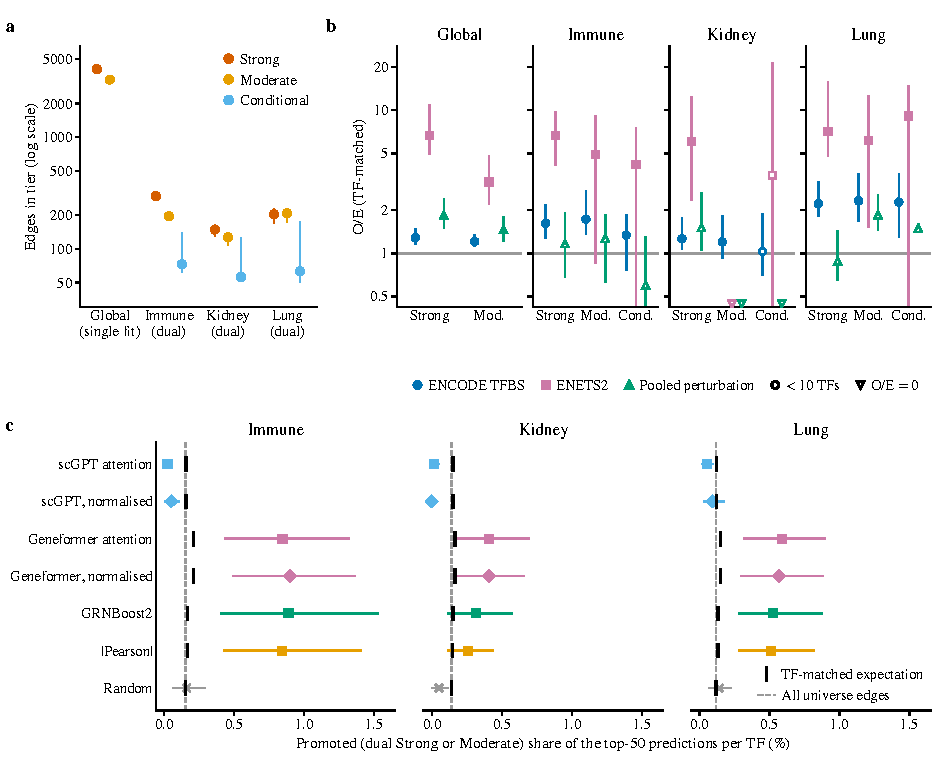
\includegraphics[width=\textwidth]{fig6_governance.pdf}
  \caption{\textbf{Claim governance.} (a) Number of edges per tier: single-fit BFDR tiers in the global universe (Strong 4{,}060, Moderate 3{,}274) and dual-universe tiers in the tissue universes (Strong/Moderate/Conditional: immune 297/196/73; kidney 149/127/56; lung 204/208/63), with 95\% intervals over posterior draws of the credibilities (tissue universes). (b) Held-out positives in each tier relative to the TF-matched expectation, with 95\% TF-bootstrap intervals (open markers: fewer than 10 evaluable TFs; triangles: no positive observed; intervals reaching 0 are cut at the axis). Global universe, Strong tier: ENCODE 1.29 [1.16, 1.48], ENETS2 6.67 [4.88, 10.95], pooled perturbation 1.85 [1.49, 2.43]; Moderate tier: 1.21 [1.11, 1.35], 3.16 [2.21, 4.80], 1.47 [1.21, 1.81]. (c) Share of each method's top-50 predictions per TF that are promoted (95\% TF-bootstrap intervals), against the share expected if the method picked random targets of the same TFs (bars) and the share among all universe edges (dashed). scGPT attention: immune 0.03\% vs 0.16\% expected; Geneformer attention: immune 0.85\% vs 0.21\% expected; GRNBoost2: immune 0.89\% vs 0.17\% expected.}
  \label{fig:governance}
\end{figure}


\paragraph{Foundation-model predictions.}
Almost none of the edges that the foundation models rank highest qualifies as a supported claim (\Cref{tab:methods-promoted}, \Cref{fig:governance}c).
Of the \nMethNpImm{}, \nMethNpKid{} and \nMethNpLung{} scGPT attention predictions (\nTopK{} per TF), \nMethNImm{}, \nMethNKid{} and \nMethNLung{} are promoted, against \nMethExpImm{}, \nMethExpKid{} and \nMethExpLung{} expected from their TFs (exact TF-stratified depletion test, post hoc; $p=\nMethPImm{}$, \nMethPKid{} and \nMethPLung{}).
The exact test treats the edges of a TF as exchangeable and may be anti-conservative: the uniform random score is itself depleted in kidney (\nMethNRandKid{} promoted against \nMethExpRandKid{} expected, $p=\nMethPRandKid{}$), so only the immune depletion is clear-cut.
% provenance: paper/r2/tables/tab_methods_promoted.tex generated by src/r2/paper_assets on 2026-10-15 04:06 from data/r2/tables/
%   gov_promoted_by_method.csv (modified 2026-10-14 20:11): k == 50; method == all_edges (k empty)
\begin{table}[tbp]
\centering
\small
\setlength{\tabcolsep}{4pt}
\caption{Promoted share of each method's predicted set (top 50 targets per TF) in the tissue-context universes, against the share expected from the TF composition of the set (TF-matched expectation); exact one-sided $p$ for enrichment and depletion.}
\label{tab:methods-promoted}
\begin{tabular}{@{}lrrcrccc@{}}
\toprule
Method & Predicted & \multicolumn{2}{c}{Promoted} & Expected & Ratio & \multicolumn{2}{c}{Exact $p$$^{\dagger}$} \\
\cmidrule(lr){3-4}\cmidrule(lr){7-8}
 & edges & $n$ & \% [95\% CI] & \% & & enriched & depleted \\
\midrule
\multicolumn{8}{@{}l}{\emph{Immune}} \\
All edges & 323{,}127 & 493 & 0.15 & 0.15 & 1.00 & -- & -- \\
scGPT & 7{,}900 & 2 & 0.03 [0.00, 0.06] & 0.16 & 0.16 & 1 & $3.5\times 10^{-4}$ \\
scGPT norm. & 7{,}900 & 4 & 0.05 [0.00, 0.11] & 0.16 & 0.33 & 1 & $5.6\times 10^{-3}$ \\
Geneformer & 5{,}322 & 45 & 0.85 [0.43, 1.33] & 0.21 & 4.04 & $2.6\times 10^{-15}$ & 1 \\
Geneformer norm. & 5{,}322 & 48 & 0.90 [0.49, 1.37] & 0.21 & 4.31 & $2.3\times 10^{-17}$ & 1 \\
GRNBoost2 & 7{,}204 & 64 & 0.89 [0.40, 1.53] & 0.17 & 5.28 & $1.7\times 10^{-27}$ & 1 \\
|Pearson| & 7{,}250 & 61 & 0.84 [0.43, 1.41] & 0.17 & 5.03 & $3.8\times 10^{-25}$ & 1 \\
Random & 8{,}050 & 13 & 0.16 [0.06, 0.30] & 0.15 & 1.06 & 0.46 & 0.65 \\
\addlinespace[3pt]
\multicolumn{8}{@{}l}{\emph{Kidney}} \\
All edges & 193{,}686 & 276 & 0.14 & 0.14 & 1.00 & -- & -- \\
scGPT & 5{,}300 & 1 & 0.02 [0.00, 0.06] & 0.15 & 0.12 & 1 & $2.7\times 10^{-3}$ \\
scGPT norm. & 5{,}300 & 0 & 0.00 [0.00, 0.00] & 0.15 & 0.00 & 1 & $2.9\times 10^{-4}$ \\
Geneformer & 4{,}866 & 20 & 0.41 [0.18, 0.70] & 0.17 & 2.49 & $1.9\times 10^{-4}$ & 1 \\
Geneformer norm. & 4{,}866 & 20 & 0.41 [0.18, 0.66] & 0.17 & 2.49 & $1.9\times 10^{-4}$ & 1 \\
GRNBoost2 & 5{,}384 & 17 & 0.32 [0.11, 0.58] & 0.15 & 2.10 & $3.5\times 10^{-3}$ & 1 \\
|Pearson| & 5{,}400 & 14 & 0.26 [0.11, 0.44] & 0.15 & 1.73 & $3.4\times 10^{-2}$ & 0.98 \\
Random & 5{,}700 & 3 & 0.05 [0.00, 0.12] & 0.14 & 0.37 & 0.99 & $3.7\times 10^{-2}$ \\
\addlinespace[3pt]
\multicolumn{8}{@{}l}{\emph{Lung}} \\
All edges & 343{,}512 & 412 & 0.12 & 0.12 & 1.00 & -- & -- \\
scGPT & 7{,}700 & 4 & 0.05 [0.01, 0.10] & 0.12 & 0.43 & 0.98 & $4.5\times 10^{-2}$ \\
scGPT norm. & 7{,}700 & 7 & 0.09 [0.03, 0.18] & 0.12 & 0.76 & 0.82 & 0.29 \\
Geneformer & 5{,}784 & 34 & 0.59 [0.31, 0.90] & 0.15 & 3.88 & $2.8\times 10^{-11}$ & 1 \\
Geneformer norm. & 5{,}784 & 33 & 0.57 [0.29, 0.88] & 0.15 & 3.77 & $1.2\times 10^{-10}$ & 1 \\
GRNBoost2 & 6{,}842 & 36 & 0.53 [0.28, 0.88] & 0.13 & 3.92 & $5.4\times 10^{-12}$ & 1 \\
|Pearson| & 6{,}850 & 35 & 0.51 [0.28, 0.82] & 0.13 & 3.82 & $2.3\times 10^{-11}$ & 1 \\
Random & 7{,}800 & 11 & 0.14 [0.06, 0.23] & 0.12 & 1.18 & 0.34 & 0.77 \\
\bottomrule
\end{tabular}
\par\smallskip
\begin{minipage}{\linewidth}\footnotesize
All universe edges: the whole context universe (reference row; its promoted share is the share of promoted edges in the universe and equals its TF-matched expectation by definition). Interval: 95\% TF-cluster bootstrap interval of the promoted share. Exact $p$: conditional on, for every TF, its numbers of universe, promoted and predicted edges; the test treats the edges of a TF as exchangeable and is anti-conservative when they are dependent.

$^{\dagger}$\,Post hoc: defined after the held-out data had been examined.
\end{minipage}
\end{table}

Geneformer attention and GRNBoost2 predictions are promoted \nMethRatioMinW{} to \nMethRatioMaxW{} times more often than expected from their TFs, but still below \nMethFracBound{}\% of their predictions.
The scGPT attention ranking largely reproduces the attention every target would receive if each cell attended uniformly to its expressed genes: the \nTopK{} top targets per TF overlap with those of this $1/L$ null by \nFmOverlapPctMin{}--\nFmOverlapPctMax{}\%, against \nFmOverlapRandPctMin{}--\nFmOverlapRandPctMax{}\% for a random ranking, and on held-out ENCODE scGPT attention is not enriched beyond the null (post hoc comparison; ratio \nFmEncRatioScMin{}--\nFmEncRatioScMax{}; Supplementary Table~\ref{tab:S-fm-heldout}); on the stricter ENCODE subset it exceeds the null only in kidney (\nFmStrictRatioScKid{} [\nFmStrictRatioScKidLo{}, \nFmStrictRatioScKidHi{}], \nFmStrictScKidTfs{} TFs).
scGPT attention stays below a random score on ENCODE for predicted sets of \nTopKSensLo{}, \nTopK{} and \nTopKSensHi{} targets per TF, and restricting attention to pairs co-observed in at least \nFmMinCoobs{} cells does not remove the null's imprint: the restriction keeps only \nFmCoobsRetPctMin{}--\nFmCoobsRetPctMax{}\% of the scGPT predicted set, and the restricted set still shares \nFmCoobsOvPctMin{}--\nFmCoobsOvPctMax{}\% of its targets with the $1/L$ null, against at most \nFmCoobsOvRandPctMax{}\% for a random ranking (Supplementary Table~\ref{tab:S-fm-sens}).
On the ChIP references and the pooled perturbation reference, Geneformer attention exceeds its null only on ENETS2 (post hoc comparison; ratio \nFmEnetRatioGfImm{} [\nFmEnetRatioGfImmLo{}, \nFmEnetRatioGfImmHi{}] in immune, \nFmEnetRatioGfKid{} in kidney).
\emph{Interpretation:} attention weights of scGPT, extracted as is common practice, reflect how many genes each cell expresses rather than regulatory relationships; Geneformer attention carries a weak signal for the specific ChIP reference.

\paragraph{Sensitivity of the tiers.}
Over the threshold grid (Supplementary Table~\ref{tab:S-gov-grid} and Fig.~\ref{fig:S-gov-grid}) the promoted set grows from \nGovQmImmMin{} to \nGovQmImmMax{} edges in immune as the Moderate threshold moves from \nGovQmGridMin{} to \nGovQmGridMax{}, with stable ENCODE enrichment (\nGovQmOeImmMin{}--\nGovQmOeImmMax{}); the Strong threshold cannot change the promoted set under the primary rule, by construction.
A rule one tier stricter (\Cref{sec:governance}) promotes \nGovStrictImm{}, \nGovStrictKid{} and \nGovStrictLung{} edges; one tier more lenient leaves the promoted set unchanged, because no edge is Strong under one fit and below Moderate under the other.
Posterior-mode instead of posterior-mean credibility changes it little (Jaccard \nGovMapJMin{}--\nGovMapJMax{}).
EM credibility promotes \nGovEmNMin{}--\nGovEmNMax{} edges per tissue.
At equal set size (post hoc), the Family-HB tiers, EM, the number of reporting annotators and the held-in DoRothEA level give overlapping held-out enrichment (ENCODE \nGovSmEncImmMin{}--\nGovSmEncImmMax{} in immune), so what governance adds is an explicit, model-based error statement with posterior uncertainty, not a better ranking.
In the simulations of \Cref{sec:res-fit,sec:res-hubs} that statement is approximately calibrated when the dominant mode is the right one: the realised false discovery rate of the Strong tier is \nSimFdrRightMin{}--\nSimFdrRightMax{} in the mode simulations, against a nominal \nSimClaimed{}.
It is somewhat anti-conservative in the hub simulations without copying (\nSimHbFdrNoCopyMin{}--\nSimHbFdrNoCopyMax{}) and when the class composition depends on literature coverage (\nSimFdrStratImm{} in the immune design with stratum-dependent class weights, \nSimFdrStratGlob{} in the global design), clearly anti-conservative when false claims are copied around hub TFs (\nSimHbFdrCopy{}), and of no help when the wrong mode is selected (\nSimFdrWrong{}).

\paragraph{Concentration.}
The promoted sets concentrate on well-studied TFs: the most frequent TF holds \nGovTopImmPct{}\% (\nGovTopTfImm{}, immune), \nGovTopKidPct{}\% (\nGovTopTfKid{}, kidney) and \nGovTopLungPct{}\% (\nGovTopTfLung{} and SPI1, tied, lung) of the promoted edges, against at most \nGovTopEligBound{}\% of the eligible edges.
A deconcentration operating point chosen without validation data (\nDecBudgetImm{}, \nDecBudgetKid{} and \nDecBudgetLung{} edges, penalty $\lambda=$ \nDecAlphaImm{}, \nDecAlphaKid{} and \nDecAlphaLung{}; its selection rule was fixed after held-out results of other analyses existed) lowers the share of the most frequent TF to \nDecTopPctMin{}--\nDecTopPctMax{}\% while keeping a mean credibility of \nDecCredMin{}--\nDecCredMax{}; its held-out ENCODE enrichment (\nDecOeMin{}--\nDecOeMax{}) rests on \nDecNevalMin{}--\nDecNevalMax{} evaluable edges and is not distinguishable from that of the undeconcentrated set.


\subsection{Hub concentration reflects the evidence, and in simulation modelling dependence reduces it relative to conditional-independence scores}\label{sec:res-hubs}

Is the concentration of promoted edges on hub TFs a property of the estimator or of the evidence? Empirically, \nHubSharePctMin{}--\nHubSharePctMax{}\% of the Family-HB Strong set falls in the top fifth of TFs by literature degree, which holds \nHubPosPctMin{}--\nHubPosPctMax{}\% of the held-out positives, an over-promotion index of \nHubIdxEnc{} [\nHubIdxEncLo{}, \nHubIdxEncHi{}] for ENCODE, \nHubIdxEnet{} [\nHubIdxEnetLo{}, \nHubIdxEnetHi{}] for ENETS2 and \nHubIdxPert{} [\nHubIdxPertLo{}, \nHubIdxPertHi{}] for perturbation (\Cref{fig:hubs}a).
Every estimator and combination rule lies in the same range (\nHubAllMin{}--\nHubAllMax{} for their top \nEvalK{} edges, against \nHubRandMin{}--\nHubRandMax{} for a random score), so the index cannot separate estimators on real data.
% generated by src/r2/paper_assets (make_paper_assets.py figures); do not edit by hand
% provenance: fig7_hubs generated by src/r2/paper_assets on 2026-10-15 04:07 from data/r2/tables/
%   heldout_degree_calibration.csv (modified 2026-10-14 20:08): reference in {encode, enets2, pert_pooled}; (score, set) in (family_hb, strong_bfdr05), (em, top500), (fisher, top500), (dorothea_level_heldin, top500), (random, top500)
%   sim_hub_summary.csv (modified 2026-10-14 20:37): set_rule = size_matched, metric in {over_promotion_lit_q5, over_promotion_top_decile}; methods oracle, family_hb, em, dependence, fisher, stouffer, majority, union, vote_fraction; set_rule = size_matched, metric = set_size, method = family_hb
%   (constants): FEW_TFS from r2.heldout_eval
\begin{figure}[tbp]
  \centering
  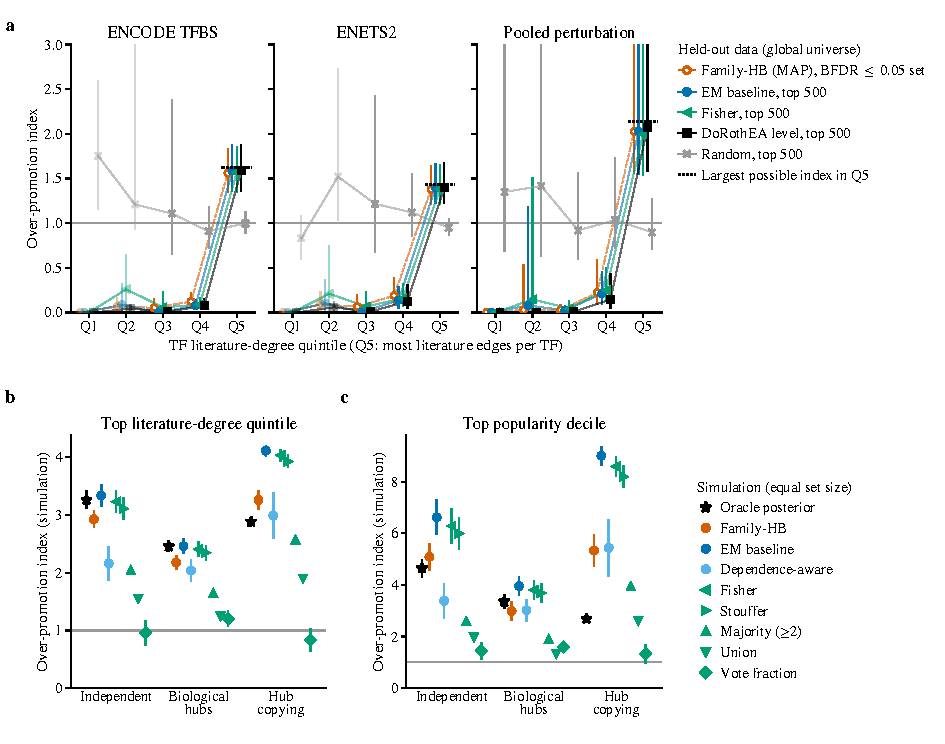
\includegraphics[width=\textwidth]{fig7_hubs.pdf}
  \caption{\textbf{Over-promotion of well-studied TFs.} The over-promotion index of a selected set for a group of TFs is the share of the set in the group divided by the share of positives (a) or of true edges (b, c) in the group (1: proportional to the positives; in (b, c) the oracle posterior shows the level the evidence supports). (a) Held-out data, global universe: index by quintile of TF literature degree for the Family-HB (MAP) BFDR $\leq 0.05$ set and for the top 500 edges of selected scores, with 95\% TF-bootstrap intervals holding the set fixed (faded (post hoc): fewer than 5 evaluable TFs in the quintile). Literature edges per TF in quintiles Q1--Q5: 1--2, 3--6, 7--17, 18--54, 55--1{,}444. The top quintile holds 96\% of the Family-HB set but 62\% of ENCODE positives; index of the Family-HB set in the top quintile: ENCODE 1.56 [1.34, 1.84], ENETS2 1.38 [1.20, 1.65], pooled perturbation 2.03 [1.55, 3.11]; random top 500 on ENCODE: 1.00 [0.88, 1.13]. In the top quintile the index cannot exceed 1/(share of positives) (dotted; ENCODE TFBS 1.62; ENETS2 1.43; Pooled perturbation 2.14), so every informative score is near this ceiling and panel (a) does not separate estimators; the sets also differ in size. (b, c) Simulation with known truth (20 replicates per scenario; mean with 95\% interval over replicates): index of sets of the size of the Family-HB BFDR $\leq 0.05$ set at TFs in the top literature-degree quintile (b) and in the top popularity decile (c), relative to the true edges. Under hub-concentrated copying (b): oracle posterior 2.89 [2.80, 2.97], Family-HB 3.26 [3.10, 3.42], EM 4.11 [4.02, 4.20], Fisher 4.03 [3.93, 4.14]. Family-regularized coincides with EM to two decimals and is not shown. All simulation rows are post hoc.}
  \label{fig:hubs}
\end{figure}

With known truth (the hub-bias simulation of \Cref{sec:inference}, \nSimHubNrep{} replicates per scenario; post hoc) even the posterior of the true generative model concentrates on popular TFs, because true edges of little-studied TFs are rarely reported: for sets of the size of the Family-HB Strong set its over-promotion index is \nSimOrIdxQMin{}--\nSimOrIdxQMax{} in the top literature-degree quintile (\Cref{fig:hubs}b) and \nSimOrIdxMin{}--\nSimOrIdxMax{} in the top popularity decile (\Cref{fig:hubs}c, Supplementary Table~\ref{tab:S-simhub}).
At equal set size, Family-HB is slightly less hub-concentrated than this oracle on the quintile scale, which is the scale of the real-data index, when popular TFs are also biologically more connected (\nSimHbOrQBio{} [\nSimHbOrQBioLo{}, \nSimHbOrQBioHi{}]) or when nothing distinguishes popular TFs (\nSimHbOrQNull{} [\nSimHbOrQNullLo{}, \nSimHbOrQNullHi{}]), and more concentrated when false literature claims are copied preferentially around popular TFs ($+$\nSimHbOrQCopy{} [\nSimHbOrQCopyLo{}, \nSimHbOrQCopyHi{}]).
In the top popularity decile the copying effect is much larger ($+$\nSimHbOrCopy{} [\nSimHbOrCopyLo{}, \nSimHbOrCopyHi{}], against \nSimHbOrBio{} [\nSimHbOrBioLo{}, \nSimHbOrBioHi{}] and $+$\nSimHbOrNull{} [\nSimHbOrNullLo{}, \nSimHbOrNullHi{}] in the other two scenarios); under copying the realised false discovery rate of the Family-HB Strong set rises to \nSimHbFdrCopy{} [\nSimHbFdrCopyLo{}, \nSimHbFdrCopyHi{}], with \nSimHbFpTopCopyPct{}\% of its false claims at top-decile TFs.
The conditional-independence scores are more hub-concentrated than Family-HB: EM and Fisher in all \nSimHubRepAll{} replicates of the three scenarios (top-decile index relative to Family-HB, EM $+$\nSimEmHbMin{} to $+$\nSimEmHbMax{}; Fisher $+$\nSimFiHbMin{} to $+$\nSimFiHbMax{}) and Stouffer in \nSimStGtN{} of them ($+$\nSimStHbMin{} to $+$\nSimStHbMax{}).
The counting rules, union, majority and vote fraction, are less hub-concentrated than Family-HB in every scenario (\nSimCountHbMin{} to \nSimCountHbMax{}), but their precision is lower by \nSimCountPrecLossMin{} to \nSimCountPrecLossMax{}, so their lower concentration reflects a less selective ranking rather than a better one.
\emph{Implication:} hub concentration is largely a consequence of how evidence is generated; in simulation, modelling within-family dependence reduces it relative to the conditional-independence scores, but no reference-only estimator removes it, and promoted edges of hub TFs should be interpreted with that in mind. The simulation uses one generator, whose burst structure resembles Family-HB, so these comparisons are indicative.


\subsection{Cross-cohort replication check}\label{sec:res-replication}

\nRepNEvalCap{} of the \nCohStudies{} perturbation studies are evaluable for TF--target edges in the global universe; Adamson perturbed no TF of the universe and Shifrut had no evaluable positives (\Cref{tab:replication}, \Cref{fig:replication}).
The power calculation fixed before any replication outcome was computed classifies Norman, Papalexi and Replogle as adequately powered (power at a \nRepTrueEnrFold{} enrichment \nRepPowMin{}--\nRepPowMax{}; minimum detectable enrichment \nRepMdeMin{}--\nRepMdeMax{}) and Dixit as underpowered and uninformative (\nRepDixitNpos{} positives; power \nRepDixitPow{}; no number of promoted edges reaches the support floor).
Within TFs, promoted edges are more often perturbation positives than other evaluable edges: stratified enrichment \nRepEnrNorman{} [\nRepEnrNormanLo{}, \nRepEnrNormanHi{}] for Norman, \nRepEnrPapalexi{} [\nRepEnrPapalexiLo{}, \nRepEnrPapalexiHi{}] for Papalexi and \nRepEnrReplogle{} [\nRepEnrReplogleLo{}, \nRepEnrReplogleHi{}] for Replogle (exact stratified $p=\nRepPNorman{}$, \nRepPPapalexi{} and \nRepPReplogle{}), and none for Dixit.
% provenance: paper/r2/tables/tab_replication.tex generated by src/r2/paper_assets on 2026-10-15 04:06 from data/r2/tables/
%   rep_units.csv (modified 2026-10-14 20:15): universe == global & level == study & comparator == universe
%   rep_power.csv (modified 2026-10-08 17:40): universe == global & level == study & comparator == universe
%   rep_pass_rates.csv (modified 2026-10-14 20:15): universe == global & level == study & comparator == universe
%   eval_analysis_decisions.csv (modified 2026-10-15 01:28): module == replication, id == rep_attainable; module == replication, id == rep_wrongtf; module == replication, id == rep_responsiveness; module == replication, id == rep_boot_clusters
%   replication.py.csv: MIN_BOOT_CLUSTERS (TFs needed for a bootstrap interval)
\begin{table}[tbp]
\centering
\small
\setlength{\tabcolsep}{2.4pt}
\caption{Cross-cohort replication check in the global universe, per independent study (Dixit 2016, \citet{dixit2016perturb}; Adamson 2016, \citet{adamson2016multiplexed}; Shifrut 2018, \citet{shifrut2018genome}; Norman 2019, \citet{norman2019exploring}; Papalexi 2021, \citet{papalexi2021characterizing}; Replogle 2022, \citet{replogle2022mapping}). Design quantities were computed and locked before any replication outcome: power of the exact stratified test against a 2-fold enrichment, minimum detectable enrichment (MDE) and support floor (promoted evaluable edges for 80\% power). Outcome: stratified O/E with 95\% TF-cluster bootstrap interval, Mantel--Haenszel odds ratio and exact one-sided $p$.}
\label{tab:replication}
\begin{tabular}{@{}lrrrrrcrclrr@{}}
\toprule
Study & Promoted & \multicolumn{3}{c}{Design (locked)} & Margins & \multicolumn{4}{c}{Outcome} & \multicolumn{2}{c}{Controls (O/E)} \\
\cmidrule(lr){3-5}\cmidrule(lr){6-6}\cmidrule(lr){7-10}\cmidrule(lr){11-12}
 & evaluable & Power & MDE & Floor & Max. & O/E & MH & $p$ & Result & Wrong & Resp.- \\
 & edges & & & & O/E$^{\dagger}$ & [95\% CI]$^{\dagger}$ & OR & & & TF$^{\dagger}$ & strat.$^{\dagger}$ \\
\midrule
Dixit 2016 & 364 & 0.03 & 27.40 & $\infty$ & 136.47 & \begin{tabular}[t]{@{}c@{}}0.00\\[-1pt]{\scriptsize --}\end{tabular} & 0.00 & 1 & \begin{tabular}[t]{@{}l@{}}under-\\powered\end{tabular} & 5.80 & 0.00 \\
Adamson 2016 & 0 & \multicolumn{10}{l}{\emph{non-evaluable: no perturbed TF of the universe tested}} \\
Shifrut 2018 & 8 & \multicolumn{10}{l}{\emph{non-evaluable: no evaluable TF positives}} \\
Norman 2019 & 220 & 1.00 & 1.39 & 40 & 4.28 & \begin{tabular}[t]{@{}c@{}}1.95\\[-1pt]{\scriptsize [1.64, 2.45]}\end{tabular} & 3.27 & $1.9\times 10^{-14}$ & pass & 1.55 & 1.25 \\
Papalexi 2021 & 571 & 1.00 & 1.41 & 109 & 7.50 & \begin{tabular}[t]{@{}c@{}}2.24\\[-1pt]{\scriptsize [1.72, 4.86]}\end{tabular} & 3.64 & $3.1\times 10^{-16}$ & pass & 1.40 & 1.41 \\
Replogle 2022 & 536 & 0.99 & 1.56 & 184 & 12.06 & \begin{tabular}[t]{@{}c@{}}1.57\\[-1pt]{\scriptsize [1.12, 4.86]}\end{tabular} & 2.07 & $7.1\times 10^{-4}$ & pass & 1.18 & 1.34 \\
\bottomrule
\end{tabular}
\par\smallskip
\begin{minipage}{\linewidth}\footnotesize
Pass (O/E $\geq$ 1.5 and $p \leq$ 0.05): 3 of 4 evaluable studies (Wilson 95\% CI 0.30--0.95; a study below its support floor is reported as underpowered, not as a failure, but counts as not passing in this rate); 3 of 3 adequately powered studies (0.44--1.00).

Intervals$^{\dagger}$: TF-cluster bootstrap within the study, given only for studies with at least 5 TFs; --, no interval: fewer TFs, or every resample gives the same O/E (Dixit 2016).

Exact $p$: one-sided exact test conditional on the margins of every (cohort, TF) stratum; it treats the edges of a stratum as exchangeable and is anti-conservative when targets of one TF are dependent, so the TF-cluster bootstrap intervals carry the inference.

Floor $\infty$: no number of promoted edges reaches the target power. Max.\ O/E: largest O/E the margins allow. Wrong-TF: O/E when each promoted edge is scored against the perturbation of a different TF of the same cohort (specificity control). Resp.-strat.: O/E with strata additionally defined by target responsiveness (share of perturbations in which the target responds).

$^{\dagger}$\,Post hoc: defined after the held-out data had been examined.
\end{minipage}
\end{table}

The exact test conditions on the (cohort, TF) strata and treats the target genes within a stratum as exchangeable; targets of one TF are not independent, so these $p$-values are anti-conservative and serve as a screen, while the TF-cluster bootstrap intervals carry the inference.
\nRepPassAllNCap{} of \nRepPassAllD{} evaluable studies pass the endpoint (Wilson interval [\nRepPassAllLo{}, \nRepPassAllHi{}]); the fourth, Dixit, is reported as underpowered rather than as a failure, but it stays in the denominator of this rate, and \nRepPassPowN{} of \nRepPassPowD{} adequately powered studies pass ([\nRepPassPowLo{}, \nRepPassPowHi{}]).
Dropping the most influential TF leaves enrichments of \nRepDropTopMin{}--\nRepDropTopMax{}.
% generated by src/r2/paper_assets (make_paper_assets.py figures); do not edit by hand
% provenance: fig8_replication generated by src/r2/paper_assets on 2026-10-15 04:07 from data/r2/tables/
%   rep_units.csv (modified 2026-10-14 20:15): level = study, comparator = universe, status = evaluable
%   rep_prior_sensitivity.csv (modified 2026-10-14 20:18): level = study, parameter in {mu, theta_new}
%   rep_pass_rates.csv (modified 2026-10-14 20:15): level = study, comparator = universe, subset in {all_evaluable, adequately_powered}
%   rep_power.csv (modified 2026-10-08 17:40): level = study, comparator = universe: alpha, true_enrichment, target_power
%   eval_analysis_decisions.csv (modified 2026-10-15 01:28): module = replication: status of rep_attainable, rep_boot_clusters
%   (constants): replication_endpoint_enrichment from r2.common.PRESPECIFIED; MIN_BOOT_CLUSTERS from r2.replication
\begin{figure}[tbp]
  \centering
  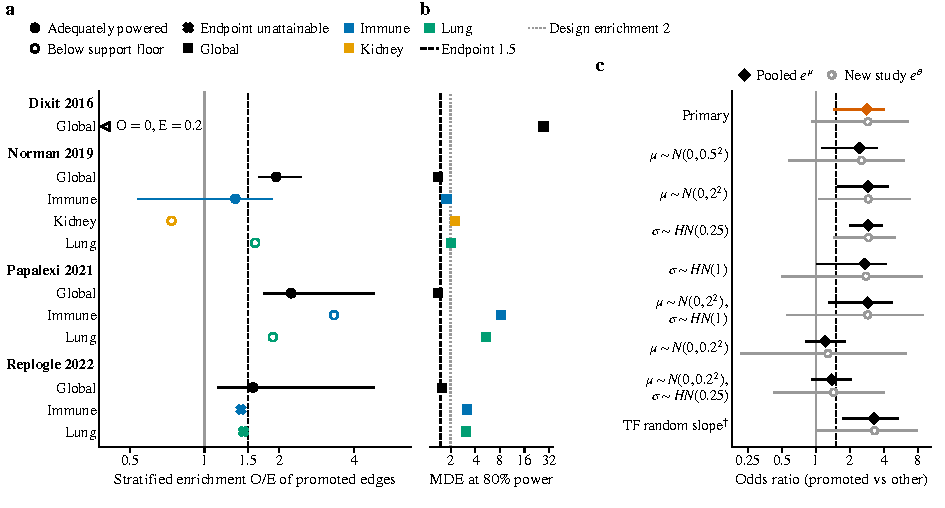
\includegraphics[width=\textwidth]{fig8_replication.pdf}
  \caption{\textbf{Cross-cohort replication check.} (a) Stratified enrichment (observed over TF-stratified expected perturbation positives among promoted evaluable edges) per study and universe (global universe primary, tissue universes secondary), with 95\% TF-bootstrap intervals where at least 5 TFs contribute (post hoc rule); intervals reaching 0 are cut at the axis. Marker shape gives the power class locked before any replication outcome was computed (filled: adequately powered; open: below the support floor); the endpoint-unattainable class (X; the positive-rate margins cannot reach the endpoint) was added post hoc; dashed line: endpoint 1.5 (non-evaluable studies omitted). Global universe: Dixit 2016: 0 observed vs 0.2 expected promoted positives (power 0.03, MDE 27.4); Norman 2019 1.95 [1.64, 2.45] (power 1.00, MDE 1.39); Papalexi 2021 2.24 [1.72, 4.86] (power 1.00, MDE 1.41); Replogle 2022 1.57 [1.12, 4.86] (power 0.99, MDE 1.56). Pass rate 3/4 evaluable studies (a study below the support floor is reported as underpowered but counts as not passing) and 3/3 adequately powered studies. (b) Minimum detectable enrichment at 80\% power and one-sided $\alpha=0.05$ from the design alone (dotted: design enrichment 2). (c) Pooled within-TF odds ratio $e^{\mu}$ and the predicted odds ratio of a new study in the Bayesian random-effects model under the primary and 7 alternative prior specifications and a model with a TF-level random slope$^{\dagger}$ (median and 95\% credible interval; N, normal; HN, half-normal; $^{\dagger}$post hoc). Primary prior: 2.82 [1.42, 4.09], $P(e^{\mu}\geq 1.5)=0.97$; sceptical prior $\mu\sim N(0,0.2^2)$: 1.21 [0.81, 1.81], $P=0.15$; across the alternative priors $P(e^{\mu}\geq 1.5)$ ranges from 0.15 to 0.99; TF random slope: 3.28 [1.71, 5.42], $P=0.99$.}
  \label{fig:replication}
\end{figure}


The check is weaker than these numbers suggest.
Promoted targets are genes that respond to many perturbations: stratifying additionally by how many other perturbed TFs a target responds to lowers the enrichments to \nRepRespNorman{}, \nRepRespPapalexi{} and \nRepRespReplogle{}, and scoring promoted targets against the responses to \emph{other} TFs already gives \nRepWrongNorman{}, \nRepWrongPapalexi{} and \nRepWrongReplogle{}, so the TF-specific excess is \nRepSpecMin{}--\nRepSpecMax{} (post hoc analyses).
After the response stratification all \nRepPassPowN{} remain below the nominal level (exact $p\le\nRepRespPMax{}$), but none reaches the endpoint of \nRepEndpoint{}.
Pooled across studies in the random-effects model, the within-TF odds ratio is \nRepMu{} [\nRepMuLo{}, \nRepMuHi{}] under the primary prior, with probability \nRepPmu{} of exceeding \nRepEndpoint{}, but the predictive interval for a new study is wide (\nRepNewLo{}--\nRepNewHi{}) and a sceptical prior centred on no effect gives \nRepSkept{} [\nRepSkeptLo{}, \nRepSkeptHi{}] (probability \nRepSkeptP{}; Supplementary Table~\ref{tab:S-rep-prior}).
Leave-$k$-out refits show the dependence on individual studies: removing one, two or three studies changes $\mu$ by \nRepLkMeanOne{}, \nRepLkMeanTwo{} and \nRepLkMeanThree{} on average (at most \nRepLkMaxOne{}, \nRepLkMaxTwo{} and \nRepLkMaxThree{}); with three studies removed a single study remains, so the last figures are single-study estimates shrunk towards the prior rather than pooled ones.
A support threshold chosen from the outcomes instead of the power calculation would be unstable: re-estimated leaving one study out, it classifies the left-out study correctly in \nRepTau{} of the cases.
\emph{Interpretation:} with \nRepPassPowD{} adequately powered studies, two of them in K562 cells, the check supports a modest, TF-specific association between promotion and perturbation response; it is not a validation.


\subsection{Sensitivity analyses and the cost of tuning on evaluation data}\label{sec:res-sensitivity}

\paragraph{Priors, evidence variants and family definitions.}
Halving or doubling the hierarchical scale priors and changing the Dirichlet concentration leave the Strong set essentially unchanged (Jaccard at least \nSensPriorMin{}; Supplementary Table~\ref{tab:S-sens-fit}).
The evidence variants matter in a structured way.
The curated-conditional variants agree with the primary (Jaccard \nSensVarKeepMin{}--\nSensVarKeepMax{}) except the panel in which the two most overlapping text-mining annotators, ExTRI and NTNU.Curated, are merged (\nSensVarMergedGlob{} global, \nSensVarMergedImm{} immune), which removes much of the co-reporting that the literature burst explains; adding the ChIP family leaves the Strong set largely unchanged (\nSensVarChipMin{}--\nSensVarChipMax{}).
Treating motif and coexpression annotators as genome-wide or requiring both endpoints, without the condition of literature support, changes the Strong set substantially (\nSensVarLeakMin{}--\nSensVarLeakMax{}) and raises held-out AP lift on ENETS2 by \nHsVarMaskMin{}--\nHsVarMaskMax{}.
Under these masks the fit sees motif and coexpression reports on edges without literature support, which in the distributed data exist only where a held-out ChIP resource supports the edge (\Cref{sec:data-annotators}), and it counts a different set of edges as uncovered; the two explanations are not separated here, and the curated-conditional model excludes both.
The family definition matters most for the size of the Strong set: grouping annotators by integrator lineage keeps \nSensGrpLinKeepPctMin{}--\nSensGrpLinKeepPctMax{}\% of the primary Strong edges but adds about as many again (a set \nSensGrpLinSizeMin{}--\nSensGrpLinSizeMax{} times as large; Jaccard index \nSensGrpLinJacMin{}--\nSensGrpLinJacMax{}), and treating every annotator as its own family removes all burst classes and reproduces the EM result, a set \nSensGrpSingSizeMin{}--\nSensGrpSingSizeMax{} times as large that contains \nSensGrpSingKeepPctMin{}--\nSensGrpSingKeepPctMax{}\% of the primary Strong edges (Jaccard \nSensGrpSingMin{}--\nSensGrpSingMax{}).
The primary Strong set is thus close to a core that every grouping retains, and the grouping decides mainly how many further edges are added.
Clustering annotators by their co-reporting pattern (post hoc) recovers the modality families exactly in the immune universe and up to one literature annotator in the global universe, where ORegAnno joins the motif cluster (adjusted Rand index \nGrpAriFullGlob{}); the Strong sets agree with the primary (Jaccard \nSensGrpDdMin{}--\nSensGrpDdMax{}), but the partition is only partly stable under resampling (mean adjusted Rand index \nGrpAriMin{}--\nGrpAriMax{} over cross-validation training folds and TF bootstraps).
On held-out data none of these choices changes the global ENETS2 AP lift by more than \nHsMaxNonLeak{}, except the two masks without the literature condition and the fit that includes the ChIP family.

\paragraph{Tuning on evaluation labels.}
Every model and evidence choice of the primary analysis was made without validation labels; to quantify what tuning on such labels would have done, we selected among \nTuneNConfigs{} configurations by perturbation AP lift on random halves of the perturbed TFs (Supplementary Table~\ref{tab:S-tuning}).
Within the hyperparameter grid and across random halves of the TFs, tuning gains nothing that transfers: \nTuneNwin{} different configurations win, and the in-sample gain over Family-HB (\nTuneIn{}) disappears on the held-out TFs (\nTuneOut{} [\nTuneOutLo{}, \nTuneOutHi{}]); with a criterion normalised for TF composition (post hoc) a gain of \nTuneNullOut{} remains, positive in \nTuneNullFracPct{}\% of the halves, so the configurations differ very little rather than not at all.
Across studies the picture differs: leaving one study out, the configuration tuned on the other studies beats Family-HB on the left-out study in all \nTuneLosoHbNfold{} folds (mean gain \nTuneLosoHbOut{}), mostly through the Dixit fold (\nTuneLosoHbExcl{} without it; post hoc subset), so label tuning on this grid can transfer between studies, although with \nTuneLosoHbNfold{} folds this is weak evidence.
Over the full grid the tuned choice is the both-endpoints observation rule in \nTuneAllFreqPct{}\% of the halves and retains \nTuneAllRetPct{}\% of its gain, partly through TF composition; across studies it retains \nTuneLosoPct{}\% of its gain, or all of it once the uninformative Dixit fold is dropped.
Choosing by cross-validated likelihood, without any label, reproduces the held-out performance of the primary model (difference \nTuneLf{}).
A selection objective that weighs dropout robustness against the perturbation reward depends on its weights and on the robustness metric: it never selects Family-HB with the $F_1$-based metric or when the combination rules are candidates, and selects it at \nTuneJointHbPrecPct{}\% of the weight settings with the precision-based metric among the latent-class models alone (Supplementary Table~\ref{tab:S-tune-weights}).

\subsection{Computation}\label{sec:res-compute}

All statistical analyses ran on one laptop (Apple M2 Pro, \nHwCores{} cores, \nHwRamGiB{}~GiB; \Cref{tab:compute}); the attention matrices were extracted beforehand, and that step is not included.
Pattern compression makes the cost of one likelihood evaluation independent of the number of edges: the \nScNRealMio{} million global edges compress to about \nScPRealApprox{} patterns in about \nScCompRealW{} second, and one evaluation of the log posterior and its gradient takes \nScVgRealMs{}~ms.
One command regenerates every table, figure and number of this paper from the stored fits in \nPipeTablesMin{}~min with at most \nPipeTablesPeakGiB{}~GiB of memory.
A full rebuild from the public inputs took about \nPipeFullHours{}~h of compute as recorded on a machine shared with other jobs, most of it in model fitting and simulation (\Cref{tab:compute}); \nPipeRecordedPct{}\% of that time consists of recorded runtimes of the original runs, and isolated re-runs of the dominant steps are \nPipeIsoRatioMin{} to \nPipeIsoRatioMax{} times faster, so the figure describes the runs as made rather than the cost on an idle machine.
As recorded, the Family-HB posterior-mode fit with \nMapRestartsHb{} restarts took \nRtMapGlob{}~s for the global universe and \nRtMapTisMin{}--\nRtMapTisMax{}~s for each tissue, and the dominant-mode NUTS fit took \nRtNutsGlobMinutes{}~min for the global universe and \nRtNutsTisMinutesMin{}--\nRtNutsTisMinutesMax{}~min for the tissues; re-run one at a time, all posterior-mode fits of the five estimators in the four universes took \nPipeMapIsoS{}~s together, and the kidney NUTS fit \nPipeNutsKidIsoMin{}~min.
In synthetic universes ten times larger (a post hoc experiment) the number of patterns grows sublinearly (exponent \nScPN{} in the number of edges), and the posterior-mode fit remains feasible: with \nScMapRestarts{} restarts it takes \nScMapTenKOne{}~s with \nScKOne{} annotators and about \nScMapTenKTwoHours{}~h (projected) with \nScKTwo{}, or about \nScMapFiftyKOneHours{}~h and \nScMapFiftyKTwoHours{}~h with the \nMapRestartsHb{} restarts used for Family-HB here.
Full NUTS becomes expensive: \nScNutsChains{} chains of \nScNutsWarm{} warm-up and \nScNutsDraw{} retained iterations are projected to take \nScNutsKOneLoHours{}--\nScNutsKOneHiHours{}~h with \nScKOne{} annotators and \nScNutsKTwoLoHours{}--\nScNutsKTwoHiHours{}~h with \nScKTwo{} (from the step-count projection, a lower bound, to the projection at the tree-depth cap; \Cref{tab:compute-scaling}), and the \nNutsChains{} chains of \nNutsWarmup{} + \nNutsDraws{} iterations used here at least \nScNutsProdMinHours{}~h, so for larger problems posterior-mode inference with Laplace or bridge-sampling summaries is the practical choice.

% provenance: paper/r2/tables/tab_compute.tex generated by src/r2/paper_assets on 2026-10-15 04:07 from data/r2/tables/
%   scale_summary.csv (modified 2026-10-14 20:38): generator in {template, independent, stress}, selected configurations
%   scale_nuts.csv (modified 2026-10-14 20:38): cid == template_real_K21 (run settings); status == projected (range over sessions)
%   fit_convergence.csv (modified 2026-10-14 19:28): universe == global & fit_id == family_hb_nuts (production NUTS run)
%   scale_environment.csv (modified 2026-10-14 20:38): keys cpu, hw.ncpu, hw.memsize (bytes)
%   pipeline_stage_timings.csv (modified 2026-10-15 04:07): selected == True; summed per stage and mode; fit_primary map and kidney NUTS: recorded vs measured wall time
%   pipeline_environment.csv (modified 2026-10-15 04:06): keys cpu, hw.ncpu, hw.memsize (bytes)
\begin{table}[tbp]
\centering
\small
\setlength{\tabcolsep}{5pt}
\caption{Wall time and peak resident memory of each stage of the analysis pipeline on the real data on one laptop (Apple M2 Pro, 10 cores, 32\,GiB), run through the single entry point \texttt{reproduce\_all.py}. Full run: every step of the stage; tables-only: the steps that regenerate the tables from the stored fits and outputs. Steps marked M were measured as isolated runs, one step process at a time with two threads; steps marked R or L are the runtimes recorded when the long fits originally ran, partly in parallel and with other thread settings on the shared machine, and make up 98\% of the full-run time. The 1-min load average of the machine (other users' jobs included) ranged 3.2--9.3 during the measured steps. Synthetic scaling: Table~\ref{tab:compute-scaling}.}
\label{tab:compute}
\begin{tabular}{@{}lrrlrr@{}}
\toprule
 & \multicolumn{3}{c}{Full run} & \multicolumn{2}{c}{Tables only} \\
\cmidrule(lr){2-4}\cmidrule(lr){5-6}
Stage & min & GiB & timing & min & GiB \\
\midrule
\multicolumn{6}{@{}l}{\emph{Data layer}} \\
Gene panels & 0.028 & 0.15 & M & 0.0068 & 0.11 \\
Annotators (committed inputs) & 0.17 & 1.6 & M & 0.17 & 1.6 \\
Evidence patterns & 0.25 & 0.99 & M & 0.25 & 0.99 \\
GRNBoost2 / GENIE3 & 71 & 5.0 & R & 0.024 & 0.21 \\
Method scores & 0.79 & 2.4 & M & 0.014 & 0.16 \\
Perturbation cohorts & 1.9 & 9.6 & R & 0.033 & 0.41 \\
Held-out ChIP & 0.84 & 4.3 & M & 0.013 & 0.15 \\
\addlinespace[3pt]
\multicolumn{6}{@{}l}{\emph{Model layer}} \\
Primary fits (MAP, NUTS) & 511 & 2.3$^{b}$ & M+R$^{a}$ & 0.16 & 0.31 \\
Sensitivity, CV, PPC, recovery & 657 & 2.0$^{b}$ & L+M+R & 0.53 & 2.0 \\
Informative-observation fits & 603 & -- & L+R$^{a}$ & -- & -- \\
Posterior modes (fits, bridge, simulation) & 688 & -- & L+R & -- & -- \\
\addlinespace[3pt]
\multicolumn{6}{@{}l}{\emph{Evaluation}} \\
Dropout robustness & 323 & 1.6$^{b}$ & L+M+R & 3.1 & 1.6 \\
Held-out evaluation & 39 & 6.6 & M & 39 & 6.6 \\
Claim governance & 0.68 & 2.3 & M & 0.68 & 2.3 \\
Posterior-mode tables, tier sensitivity & 1.0 & 3.0 & M & 1.0 & 3.0 \\
Replication check & 12 & 4.5 & M & 12 & 4.5 \\
Tuning optimism & 28 & 3.9$^{b}$ & M+R & 1.7 & 3.9 \\
Informative-observation evaluation & 11 & 8.1 & M & 11 & 8.1 \\
Hub-bias simulation & 638 & 0.23$^{b}$ & L+M+R$^{a}$ & 0.055 & 0.23 \\
Compute scaling & 384 & 9.1 & M+R & 0.050 & 0.37 \\
Informative-observation governance & 0.88 & 3.0 & M & 0.88 & 3.0 \\
\addlinespace[3pt]
\multicolumn{6}{@{}l}{\emph{Assets}} \\
Manuscript assets & 0.73 & 0.36 & M & 0.73 & 0.36 \\
\midrule
Total & 3{,}972 &  &  & 72 &  \\
\bottomrule
\end{tabular}
\par\smallskip
\begin{minipage}{\linewidth}\footnotesize
$^{a}$\,Not included in the total: no runtime is recorded for the steps Primary fits (MAP, NUTS): Laplace approximation; Informative-observation fits: evidence encoding; Hub-bias simulation: oracle check.

$^{b}$\,Memory is known only for steps that make up less than half of the stage's wall time (the long fitting steps did not record their peak memory).

Timing: M, measured as an isolated run; R, runtime recorded by the analysis script when the step originally ran (summed over its fits or replicates; no peak memory unless the script stored it); L, from the time stamps in the script's logs. All times come from a machine shared with other jobs; the recorded R and L times come from more heavily loaded runs and are the least precise. Peak memory: largest single process (GRNBoost2: summed over its dask workers). Totals: full run 66\,h of compute as recorded on the shared machine; isolated re-runs of the primary MAP fits and of the kidney NUTS fit took 3.3--3.7 times less wall time than recorded, so the total describes the runs as made rather than the cost on an idle machine; tables-only run 72\,min.
\end{minipage}
\end{table}

\begin{table}[tbp]
\centering
\small
\setlength{\tabcolsep}{4pt}
\caption{Compute scaling on synthetic evidence (no held-out data). Wall time on one laptop (Apple M2 Pro, 10 cores, 32\,GiB) for pattern compression, one log-posterior and gradient evaluation, 10 MAP restarts and a short NUTS run (2 chains $\times$ (300 warm-up + 300 draws), random starts), with peak resident memory (post hoc measurement session$^{\dagger}$).}
\label{tab:compute-scaling}
\begin{tabular}{@{}lrrrrrrrrr@{}}
\toprule
 & $N$ & $K$ & $P$ & \multicolumn{2}{c}{Compression} & Evaluation & \multicolumn{2}{c}{MAP restarts} & NUTS \\
\cmidrule(lr){5-6}\cmidrule(lr){8-9}
Data set & & & & s & MiB & ms & s & MiB & s \\
\midrule
\multicolumn{10}{@{}l}{\emph{Real-data template}} \\
$N \approx 10^{5}$ & 100{,}007 & 21 & 1{,}147 & 0.0075 & 124 & 0.57 & 14 & 584 & 62 \\
$N \approx 10^{6}$ & 1{,}000{,}008 & 21 & 4{,}964 & 0.098 & 304 & 0.87 & 28 & 658 & 527 \\
real size & 9{,}315{,}405 & 21 & 19{,}005 & 1.2 & 473 & 1.5 & 103 & 1{,}136 & 3{,}068 \\
$N \approx 10^{7}$ & 10{,}000{,}080 & 21 & 20{,}776 & 0.92 & 505 & 2.0 & 125 & 784 & 3{,}108--3{,}489$^{n}$ \\
10 $\times$ real & 93{,}163{,}242 & 21 & 88{,}131 & 9.3 & 920 & 4.2 & 685 & 1{,}093 & 6{,}693--20{,}731$^{n}$ \\
10 $\times$ real & 93{,}163{,}242 & 42 & 531{,}834 & 38 & 978 & 36 & 5{,}510$^{e}$ & 5{,}077 & 22{,}448--75{,}979$^{n}$ \\
\addlinespace[3pt]
\multicolumn{10}{@{}l}{\emph{Independent annotators}} \\
real size & 9{,}315{,}405 & 21 & 7{,}495 & 1.1 & 466 & 1.1 & 53 & 786 & -- \\
\addlinespace[3pt]
\multicolumn{10}{@{}l}{\emph{Stress (no repeated patterns)}} \\
$N \approx 10^{6}$ & 1{,}000{,}008 & 21 & 849{,}046 & 0.26 & 384 & 40 & 2{,}290$^{e}$ & 3{,}810 & 64{,}220--162{,}693$^{n}$ \\
$N \approx 10^{7}$ & 10{,}000{,}080 & 21 & 3{,}492{,}675 & 2.4 & 1{,}153 & 182 & 20{,}105$^{m}$ & 9{,}282 & 290{,}023--581{,}925$^{n}$ \\
\bottomrule
\end{tabular}
\par\smallskip
\begin{minipage}{\linewidth}\footnotesize
Real size: a synthetic universe with as many TFs and genes as the global universe, so $N$ differs from the real number of edges only by the TF self-pairs, which the real universe excludes; its number of patterns $P$ differs from the real one because its observations and reports are simulated.

$^{e}$\,MAP: extrapolated from the mean time of the restarts that finished within the time budget.

$^{m}$\,MAP not run: evaluations per restart of the first session $\times$ measured time per evaluation; a lower bound (optimiser overhead not included).

$^{n}$\,NUTS not run (time budget); range over the two measurement sessions from the projection with the leapfrog steps per iteration of the largest measured run with the same $K$ (lower end: steps per iteration grew with $N$, so this is a lower bound) to the projection at the tree-depth cap of 1{,}023 steps per iteration (upper end, the better estimate for $N \geq 10^7$).

$N$: edges; $K$: annotators; $P$: distinct observation patterns. Measured wall times are upper bounds of the undisturbed cost (machine shared with other jobs). Real-size template: observation design and fitted parameters of the global universe. The NUTS benchmark starts chains at random and is a cost measurement, not a converged fit (maximum $\widehat R$ 1.91 at real size: chains in different modes). The MAP-initialised production fit of the global universe (4 chains $\times$ (1{,}000 + 1{,}000)) took 5{,}271\,s.

$^{\dagger}$\,Post hoc: defined after the held-out data had been examined.
\end{minipage}
\end{table}

